%%%% MACRO DEFINITION %%%%

\providecommand{\pvivax}{P.~vivax}
\providecommand{\pfalciparum}{P.~falciparum}
\providecommand{\cterm}{C-terminus}
\providecommand{\nterm}{N-terminus}

\providecommand{\e}[1]{\ensuremath{\times 10^{#1}}}
\newcolumntype{P}[1]{>{\centering\arraybackslash}p{#1}}
\newcolumntype{M}[1]{>{\centering\arraybackslash}m{#1}}

\providecommand{\refimage}[1]{\figurename~\ref{fig:#1}}

%TC:macro \note [ignore]



%%%%%%%%%%%%%%%%%%%%%%%%%%%%%%%%%%%%%%%%%%%%%%%%%%%%%%%%%%%%%%%%%%%%%%%%%%%%%%%%%%%%%%%%%%%%%%%%%%%%%%%%%%%%%%%%%%%%%
%%%%%%%%%%%%%%%%%%%%%%%%%%%%%%%%%%%%%%%%%%%%%%%%%%%%%%%%%%%%%%%%%%%%%%%%%%%%%%%%%%%%%%%%%%%%%%%%%%%%%%%%%%%%%%%%%%%%%
%													BEGIN
%%%%%%%%%%%%%%%%%%%%%%%%%%%%%%%%%%%%%%%%%%%%%%%%%%%%%%%%%%%%%%%%%%%%%%%%%%%%%%%%%%%%%%%%%%%%%%%%%%%%%%%%%%%%%%%%%%%%%
%%%%%%%%%%%%%%%%%%%%%%%%%%%%%%%%%%%%%%%%%%%%%%%%%%%%%%%%%%%%%%%%%%%%%%%%%%%%%%%%%%%%%%%%%%%%%%%%%%%%%%%%%%%%%%%%%%%%%

\chapter{ZincBind --- The Database of Zinc Binding Sites} % Write in your own chapter title
\label{Chapter4}
\lhead{Chapter 4. \emph{ZincBind - The Database of Zinc Binding Sites}} % Write in your own chapter title to set the page header

\emph{Note that some of the material in this chapter has been published in the journal Database under the title `ZincBind—the database of zinc binding sites' (2019), though the values and analysis have been updated for the updated dataset.}

This project is an attempt to develop novel means of predicting Zinc Binding Sites using the known properties of previously identified Zinc Binding Sites. As such, the initial step was to create a dataset of these already-known sites.

This is an undertaking that has been performed previously on a smaller scale, several times (see Chapter 1). One of the primary reasons that the effort has been duplicated so many times is because in none of the previous dataset generations did the authors make their data publicly available in an easy-to-use resource. Therefore from the very beginning of this project, the intention was always to not \emph{just} create this dataset of Zinc Binding Sites, but also to make this database publicly available via a web resource, that would be continually updated with new sites as they become available.

This chapter will describe the creation of that dataset, and the web application that offers users access to the data: ZincBind.

\section{Data Generation}

ZincBind uses as its primary data source the Protein Databank \cite{berman2000pdb}. This contains hundreds of thousands of protein structures, a subset of which contain zinc atoms and which can be inspected to see if a zinc binding site can be identified.

The RCSB web services \cite{burley2020pdb} allow a user to query the entire databank by, among other things, the chemical formulae of its small molecules. The PDB IDs of all zinc atom containing structures can therefore be obtained by issuing a request to these web services for a \verb|ChemCompFormulaQuery| with the formula \verb|Zn|.

If the dataset is being created from scratch, each of these PDB IDs is iterated through in turn to look for zinc binding sites. If the dataset is merely being updated with new structures, only those IDs that do not already exist in the database are used.

\subsection{Structure Inspection}

The algorithm iterates through each PDB code and, for each, attempts to determine what zinc binding sites are present, if any, and saves the relevant objects to the database once its analysis is complete.

Each PDB ID is analysed within a single database transaction, meaning that the SQL statements are built up by Django throughout the analysis and then executed all at once at the end of each PDB ID analysis. This has two benefits. Firstly, it makes the whole process much faster --- there are database records for each atom in the binding site, so opening up database connections, creating a record, and closing the connection multiple times per structure is much more time consuming than just doing that once at the end. Secondly, and more importantly, if the program is interrupted in the middle of building a database, it will essentially rollback to the last fully processed PDB, rather than saving records for half-processed PDBs which could cause errors when the program is restarted.

The structures are requested from the RCSB web servers in the mmCIF file format. This, and all subsequent structure parsing and analysis, are abstracted into the atomium Python library (see Chapter 3).

The first processing step with the obtained and parsed structure, is to generate a biological assembly. The raw coordinates of the PDB structure contain the `asymmetric unit', which is often a subset or superset of the `true' biological assembly. Each PDB structure contains a list of possible biological assemblies that can be created from the chains in the asymmetric unit to make a more biologically realistic structure, and each is associated with a list of transformation matrices and calculated metrics. The $\Delta G$ of the assemblies are used to rank them, and the lowest $\Delta G$ assembly that still contains zinc is selected as the `real' biological assembly.

This step is critical. While asymmetric units are perfectly suitable if you are merely concerned with intra-chain features, they are often unsuitable for examining the interfaces between chains. Since many zinc binding sites are between chains, relying on asymmetric units would produce data that is not particularly meaningful. An example of this would be insulin, which is a hexamer of six chains and two zinc binding sites, with each chain providing one histidine residue to one of the two binding sites. For many insulin structures, the asymmetric unit contains just one chain in this hexamer and suggests that the `binding site' is a single histidine residue. Only by using the lowest energy biological assembly is the full hexamer constructed, and the true binding sites made available for analysis.

However it is important to keep in mind that, necessary though biological assembly generation is, it does introduce some problems. Many assembly instructions are simply to use a subset of the chains in the asymmetric unit, which is fine, but some require copies of chains to be created. For example, a structure that starts out with an A chain and a B chain may, in its biological assembly, have two A chains and two B chains. As there is no established protocol for generating new IDs for these chains (and since creating one would create inconsistencies with other software that uses the data in the ZincBind database, such as the NGL protein viewer), the solution used here is simply to have multiple chains with the same ID. This can cause a number of problems which will be outlined, along with their solution, as they arise in this section.

Once the correct assembly has been generated, the algorithm then checks that the resultant structure is usable, and is not just alpha carbons as some structures are. If it is such a `skeleton structure', the zinc atom(s) in that structure are saved to the database with an annotation explaining that they do not have a binding site because the PDB was unusable. Note that this is the case whenever a zinc atom is rejected --- it is still saved to the database with an explanatory annotation, because by doing this \emph{every} zinc atom in the Protein Data Bank can be accounted for in ZincBind. If this were not done, and a user tried to find a particular zinc atom from the data bank in ZincBind which had not been assigned a binding site, that user would have no way of knowing if the zinc atom was absent because ZincBind had not examined that PDB, or if it was absent because a binding site could not be assigned to it.

Any zinc atoms that are in the asymmetric unit but not the biological assembly (common in cases where the asymmetric unit is just the biological assembly repeated multiple times) are also saved to the database without a binding site, with an explanatory explanation as to why it has none, for the same reason.

The next step is to actually identify all of the binding sites. This is done as follows:

\begin{enumerate}
   \item Identify all metals in the structure. This is done using element names in atomium, but it is here that the first biological assembly related problems must be dealt with. When these assemblies are being generated, sometimes atoms end up superimposed on top of each other --- so called `special position' atoms. The correct interpretation of this is that there is just one atom here, not multiple atoms occupying the same position in space, so duplicates have to be removed. This is done with atomium by taking all atoms of a given element, comparing it with every other atom of that element, and if the distance between them is less than 1~{\AA}, one is removed.
   \item Determine the atoms which ligand each metal in the structure. All atoms within 3~{\AA} of the metal which are not carbon or hydrogen are determined, and again duplicated atoms must be removed from these using the same algorithm as above (insulin structures for example, often have a chloride ligand which would appear multiple times in the same location otherwise). Once this `cloud' of suitable liganding atoms is obtained, they are ordered by distance to the metal, and for each one a check is made that the angle formed between it, the metal, and any closer atom is not less than 45$^\circ$. If it is, the atom is removed from the set of liganding atoms as it is assumed a coordinate bond would be infeasible if there is another coordinate bond so close.
   \item Remove metals that probably aren't physiologically relevant. Sometimes a metal atom in a model is just there as a consequence of the crystallisation environment, and while it may interact with one or two residues, those residues might not be a `real' zinc binding site in the sense of being an evolutionarily selected combination of residues there specifically to bind zinc. There is no way to identify with certainty which category a given zinc atom falls into from atom coordinates alone, but ZincBind implements a filter whereby if a metal atom has fewer than three protein liganding atoms, it is discarded as probably irrelevant. Again, those atoms which are excluded at this stage are given an annotation explaining the reason, if they are zinc atoms.
   \item Merge the metals into single binding sites where necessary. So far, all metals have been considered in isolation, though in reality some of them may form co-functional units with each other. To determine if this is the case, the residues/ligands that the liganding atoms are part of are examined and, if two metals share a residue/ligand, they are assigned to the same `cluster'.
   \item Remove non-zinc binding sites. ZincBind is a database of \emph{zinc} binding sites. So far all metals have been considered because some non-zinc atoms may be part of a multi-metal site that contains zinc, so had to be included at every step. However now that the fully processed sites have been generated, those that do not contain zinc can be removed.
   \item Identify the secondary residues of each of the binding sites. This is the set of all residues which are within 3~{\AA} of a primary liganding residue. These residues are saved, along with the details of which atoms mediate these interactions. The importance of second shell residues in stabilising the primary liganding shell has been well documented, so identifying how many of these stabilising contacts exist is important information.
\end{enumerate}

See Figure~\ref{fig:zincbind-build} for an illustration of this process.

\begin{figure}
\centering
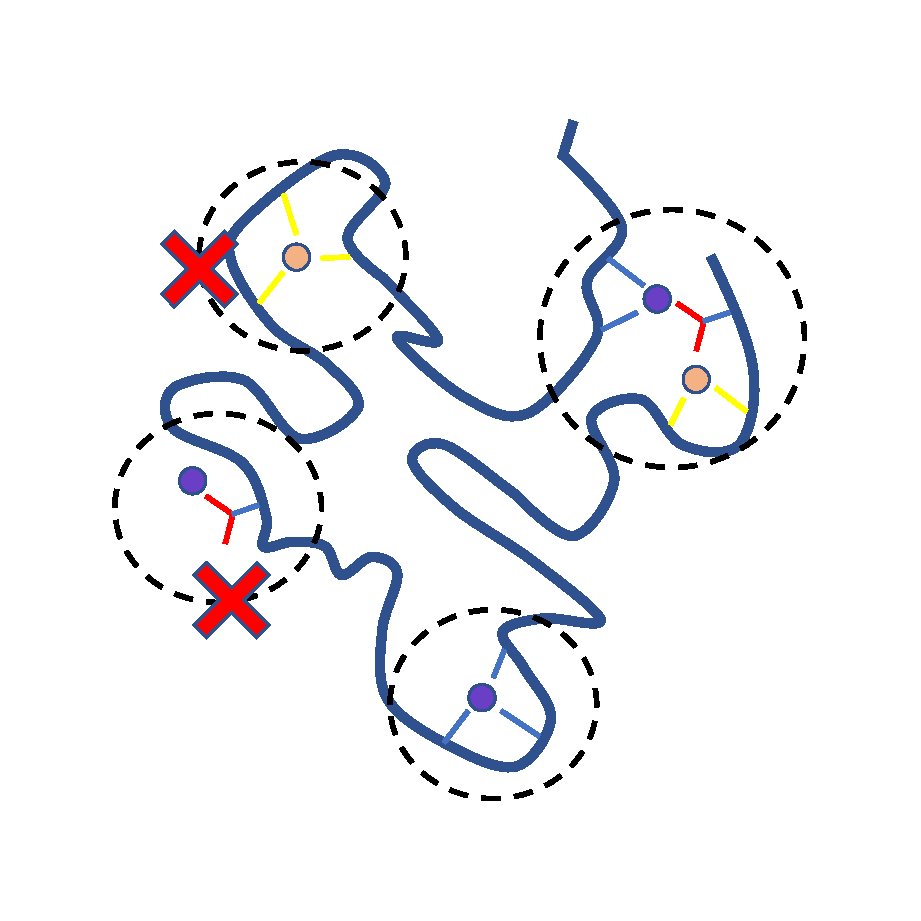
\includegraphics[width=1.0\textwidth]{Figures/zincbind-build.eps}
\caption[The ZincBind build process.]{\label{fig:zincbind-build} An illustration of how the ZincBind build algorithm identifies binding sites. Those with no zinc (top left) or too few liganding atoms (bottom left) are rejected.}
\end{figure}

Now that the zinc binding sites have been identified, they can be saved to the database. Before this is done however, the chain objects are saved to the database, as these records will be needed when the sites are saved. Any chain in the structure with a residue that is part of a binding site is saved. The sequence used is the full canonical sequence listed in the header of the structure file, not the actual sequence of residues in the model, which may contain missing residues (particularly at the ends of the sequence). These two sequences are aligned using the Smith-Waterman local alignment algorithm \cite{smith1981alignment} so that the liganding residues in the model can be identified in the full sequence, and capitalised.

\emph{Then} the sites themselves are saved to the database, along with records for any metals, residues, and residue atoms. So-called `Chain-Site Interactions' are also saved, which are essentially chains with only a single site annotated within them. While the plain chain objects saved above have residues involved in any binding site highlighted, here only the residues involved in that particular site are. This is important as chains may be involved in multiple sites, but predictive models need to know which residues contribute to \emph{single} sites.

\subsection{Equivalent Sites and Families}

The database as it stands at this point in the algorithm will be a list of zinc binding sites, where each site is considered distinct and separate from all others. This is somewhat misleading, as many proteins appear in the Protein Data Bank several times, and so the binding site(s) in those structures will appear in ZincBind several times. The binding site in (for example) Carbonic Anhydrase will appear in ZincBind many hundreds of times, yet each of these records refer to the same biological entity.

To account for this, ZincBind clusters binding sites into equivalent sites called `groups'. The first step is to cluster the zinc binding chains that were saved as part of the earlier generation process into clusters on 90\% sequence identity, using the program CD-HIT \cite{li2006cdhit}. It is assumed that chains in a CD-HIT sequence cluster are functionally equivalent.

The binding sites themselves are then clustered using these chain clusters. Two zinc binding sites are assigned to the same cluster if (1) they are associated with the same chain cluster(s), (2) they have the same residue names in the same order, and (3) their surrounding residue names are the same. These latter two steps are important to ensure that chains with two or more zinc binding sites along them do not have those binding sites incorrectly assigned to the same cluster.

A group object is stored in the database for each of these clusters, and the corresponding zinc binding sites are linked with them. Thus ZincBind stores individual zinc binding sites as they occur in the Protein Data Bank, and unique zinc binding sites in the form of groups.

Binding sites and groups form two components of the three-part hierarchy of data in ZincBind, the third being the family. Each binding site is given an alphanumerical code based on its residue content and count --- so, for example, binding sites with three histidine residues are `H3', those with two histidines and two cysteine residues are C2H2, and so on. These make up the `family' to which the binding site belongs. Binding sites are clustered into groups, which are in turn clustered into families based on residue content.

\section{The ZincBind Web Resource}

As already noted, the creation of this dataset was intended to serve both as the primary dataset of this project, and as a publicly available resource. This resource is called ZincBind, and is available over the web.

The database is accessible via a GraphQL API, which allows any specific object, or set of related objects, to be requested in a single HTTP request (see Figure~\ref{fig:zincbind-api-example}). This is available at \url{api.zincbind.net} and is the primary means of obtaining data from ZincBind in an automated fashion. As outlined in Chapter 2, this is created using the Python web framework Django (particularly its Object Relational Management system) and the GraphQL library graphene.

\begin{figure}
\centering
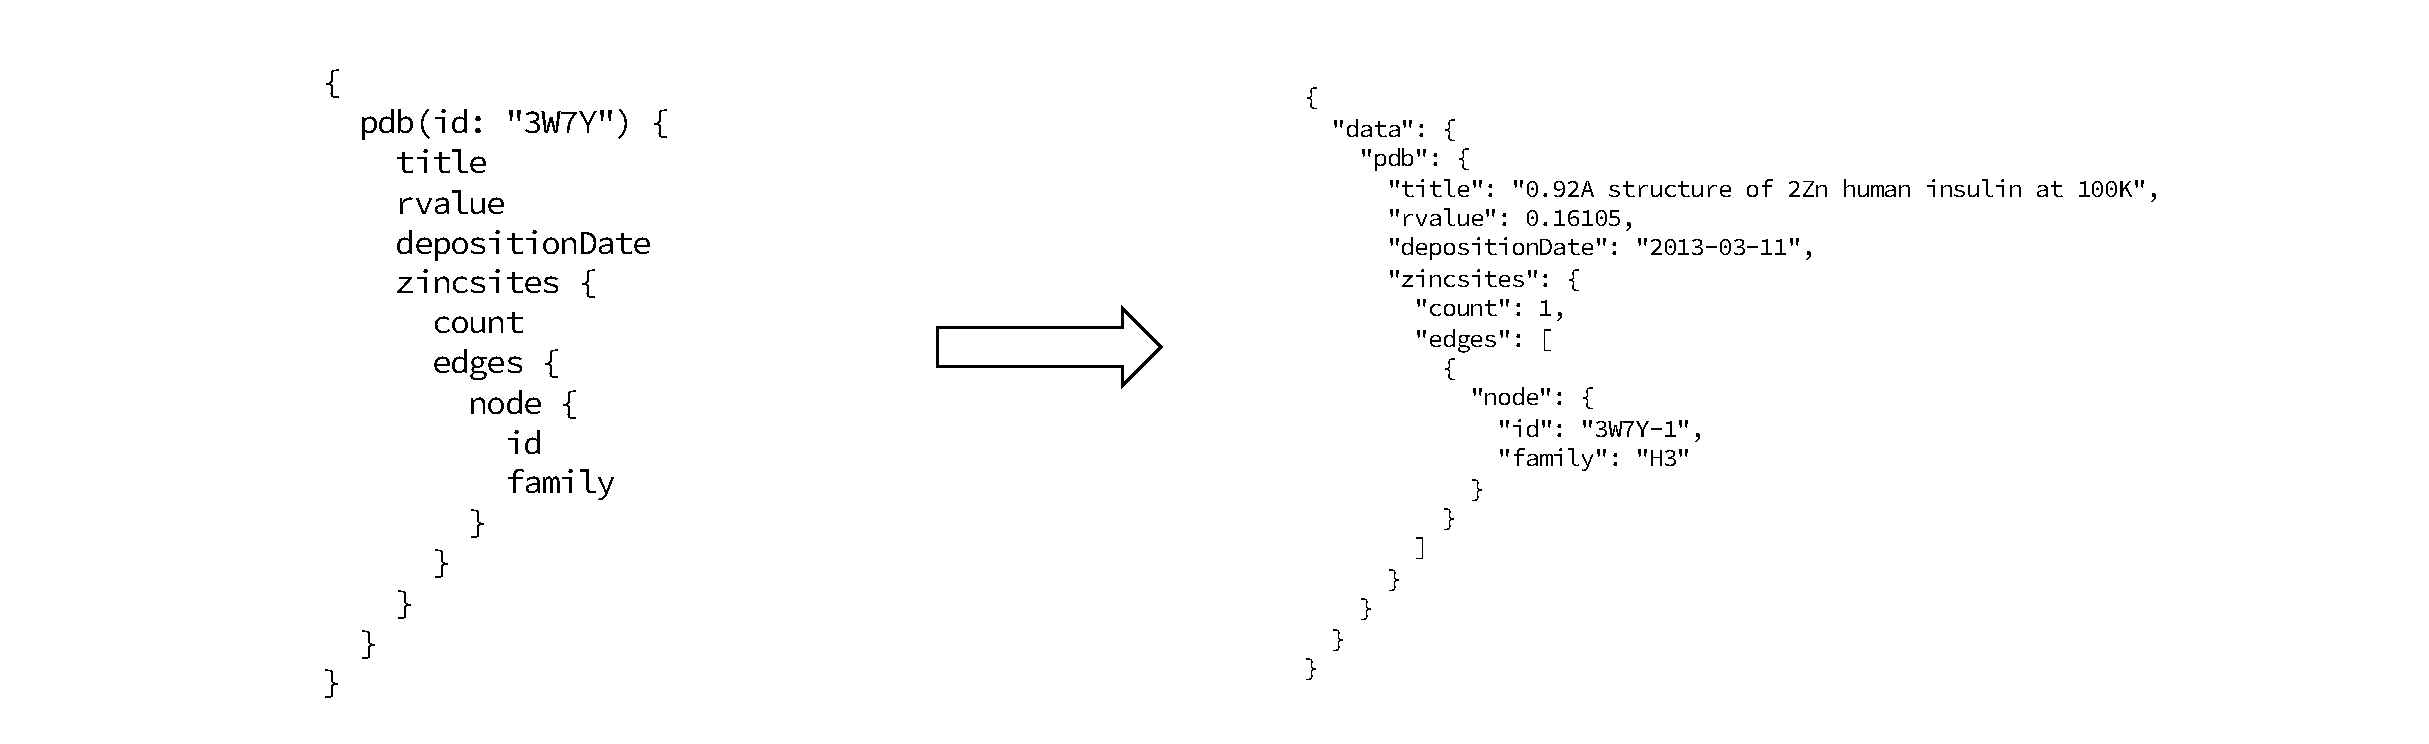
\includegraphics[width=1.0\textwidth]{Figures/zincbind-api-example.eps}
\caption[An example of a ZincBind GraphQL API query.]{\label{fig:zincbind-api-example} An example of a ZincBind GraphQL API query, in this case for a \texttt{PDB} object.
There requesting all the zinc binding sites within that \texttt{PDB} --- there is
one in this case. In this case the fields \texttt{id} and \texttt{family} are
requested for each, though they also have other fields.}
\end{figure}

More accessibly for casual browsing, there is also a website available at \url{zincbind.net}. This is a lightweight web frontend that interacts with the database via the GraphQL API and presents it to the user graphically. It is a responsive, mobile-first layout created with the front-end framework `react', that adapts to different screen sizes.

The home page (see Figure~\ref{fig:zincbind-homepage}) contains a short, clear statement of what ZincBind is (a ``database of zinc binding sites, automatically generated from the Protein Data Bank") as well as a brief overview of its key metrics: number of unique binding sites, total number of binding sites, and the number of PDB files the sites are derived from.

\begin{figure}
\centering
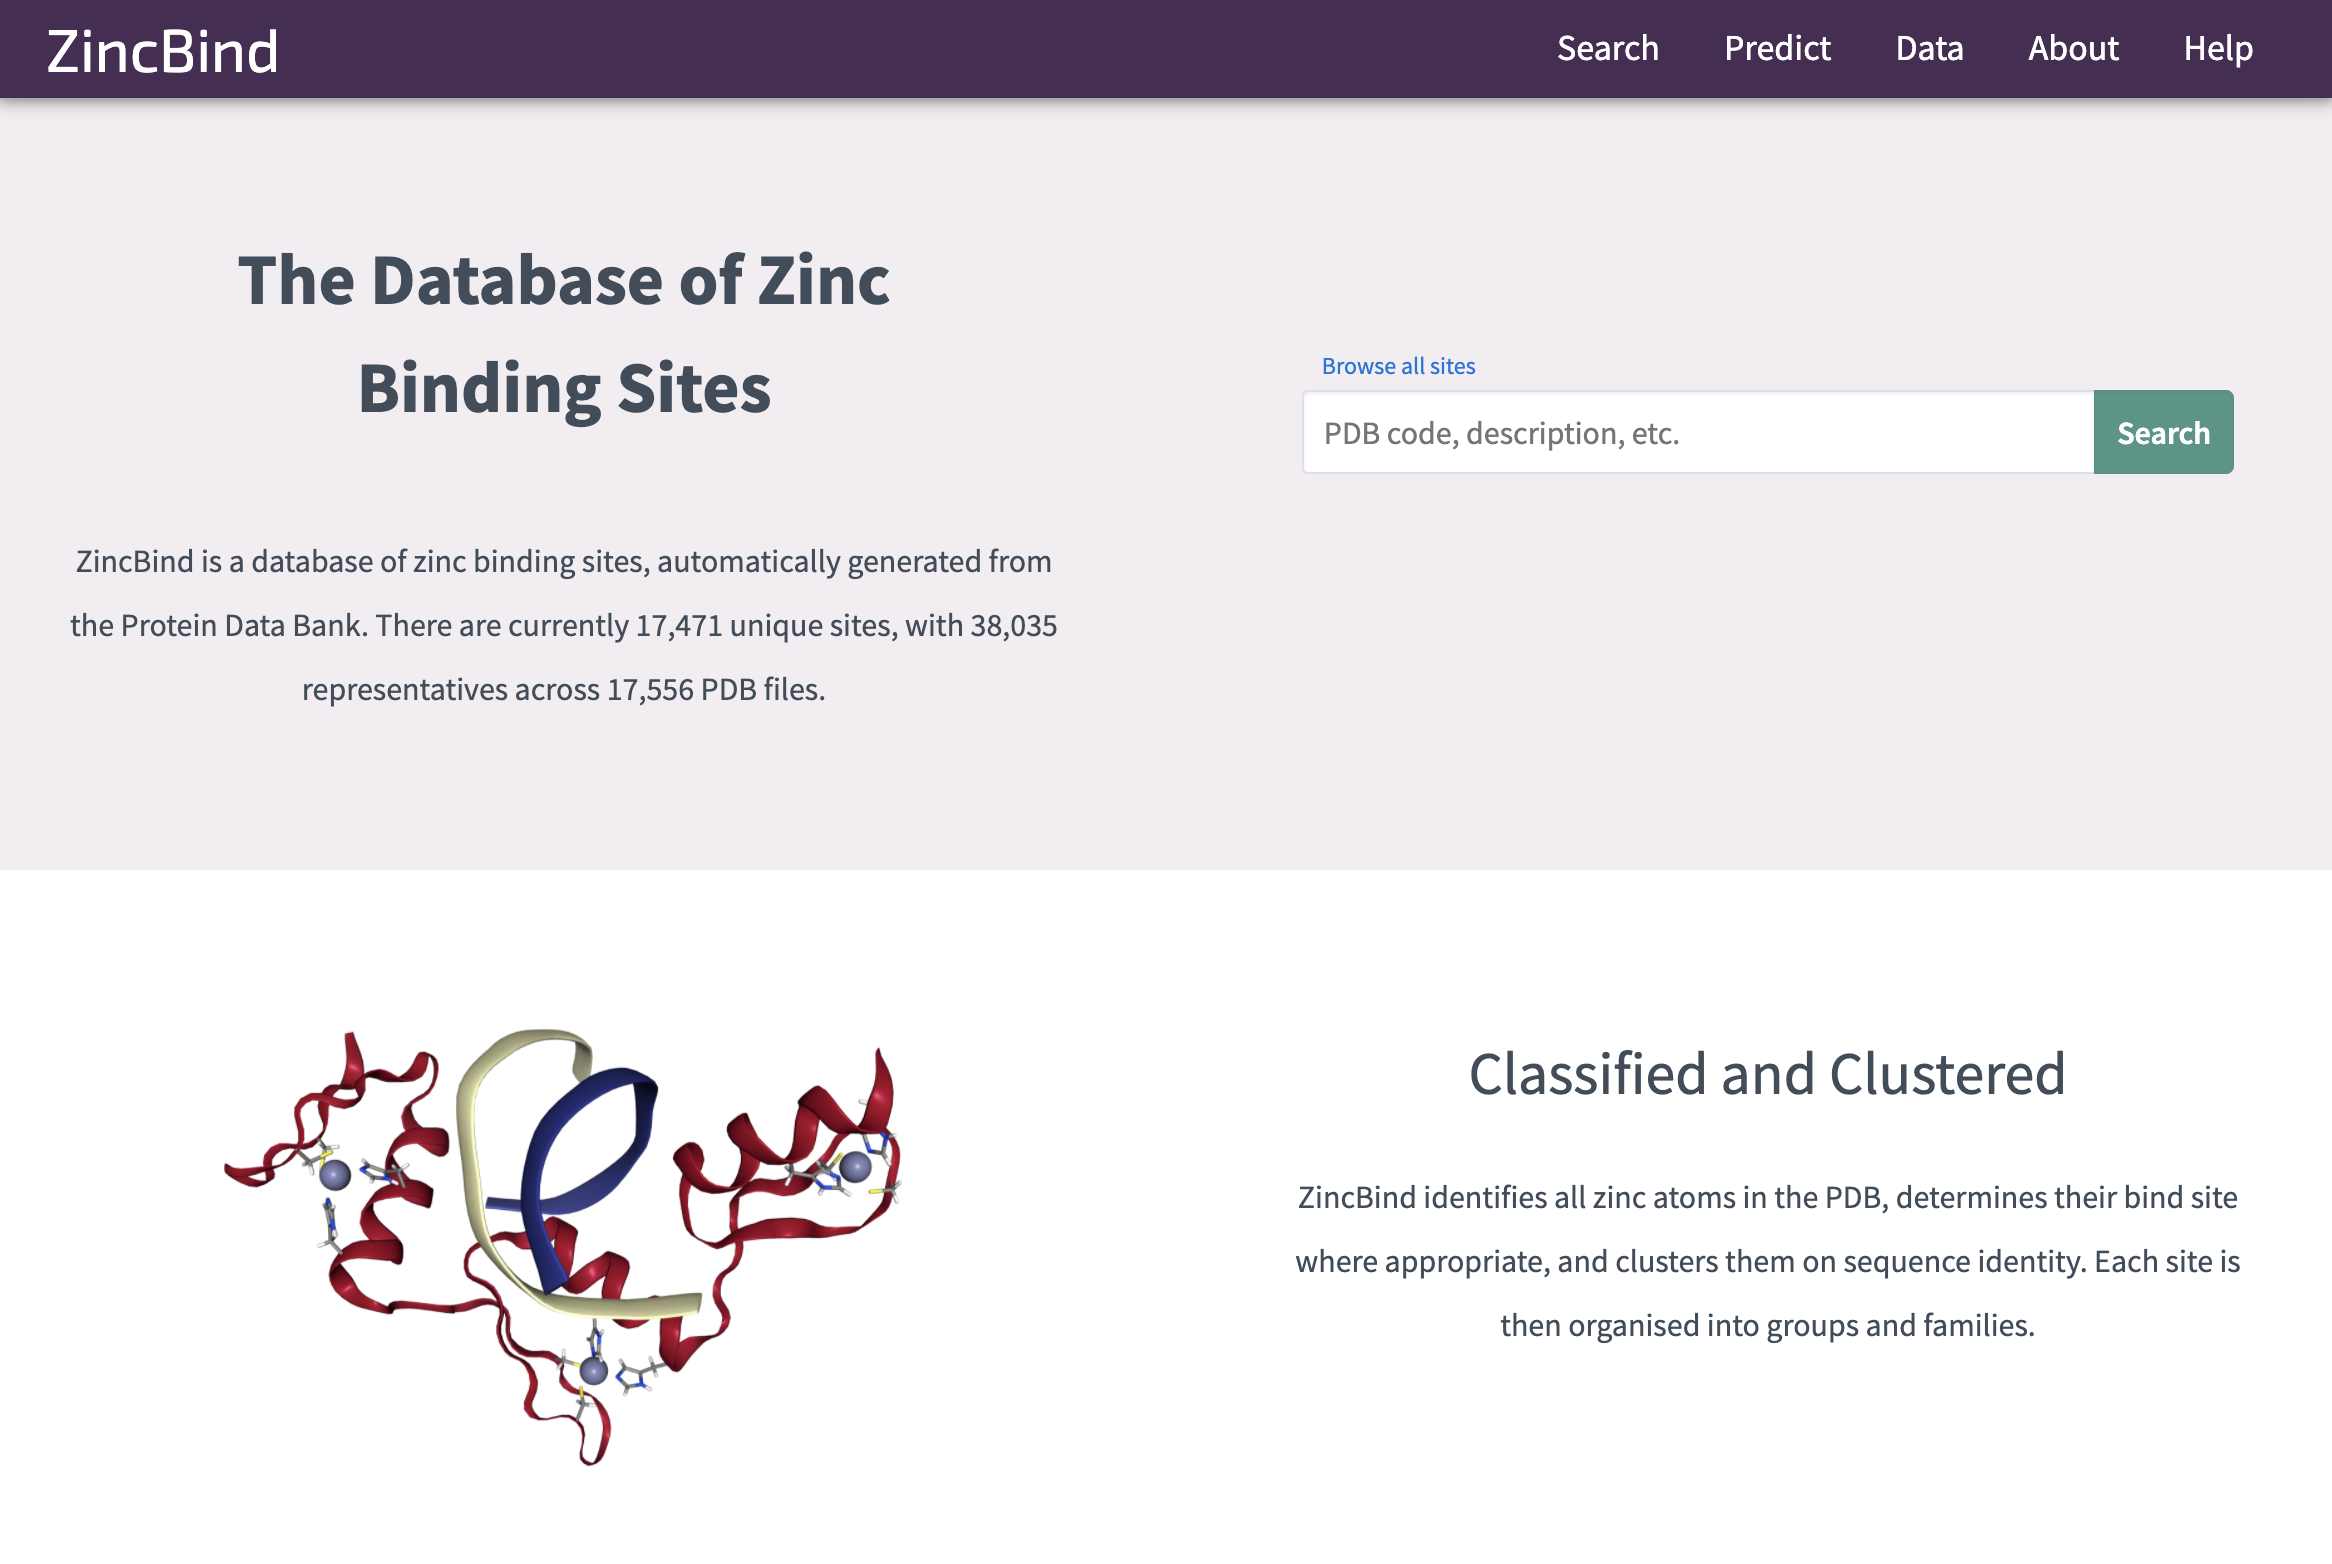
\includegraphics[width=1.0\textwidth]{Figures/zincbind-homepage.eps}
\caption[The home page of ZincBind.]{\label{fig:zincbind-homepage} The home page of ZincBind, showing the
overview statistics in the top-left, and the quick search text box in the top right.
The menu bar at the top collapses on small screen widths, making them accessible via a
drop-down menu on mobile.}
\end{figure}

Searching of the database can be done in one of four ways. Firstly, from the home page, the user can enter a search term that will be used to search multiple PDB fields at once: title, PDB code, classification, etc. This is for users who just want to find entries that have any relation to a given term at all, and provides an easy, low-friction way for a user to submit a search immediately.

Secondly, the user can navigate to the Advanced Search page (see Figure~\ref{fig:zincbind-search}), where they can specify a more precise search by one or more PDB fields. This also allows searching by numeric cutoffs, such as for PDBs better than a certain resolution or deposited after a certain date --- essentially any of the PDB metrics that are stored in the database.

Thirdly, via this same page they can search for specific binding sites rather than for containing PDBs. The user can pick the same metrics as for PDBs (sites in PDBs better than a certain resolution, with a certain classification, etc.) as well as site-specific metrics, such as sites of a particular family, or containing particular residues.

\begin{figure}
\centering
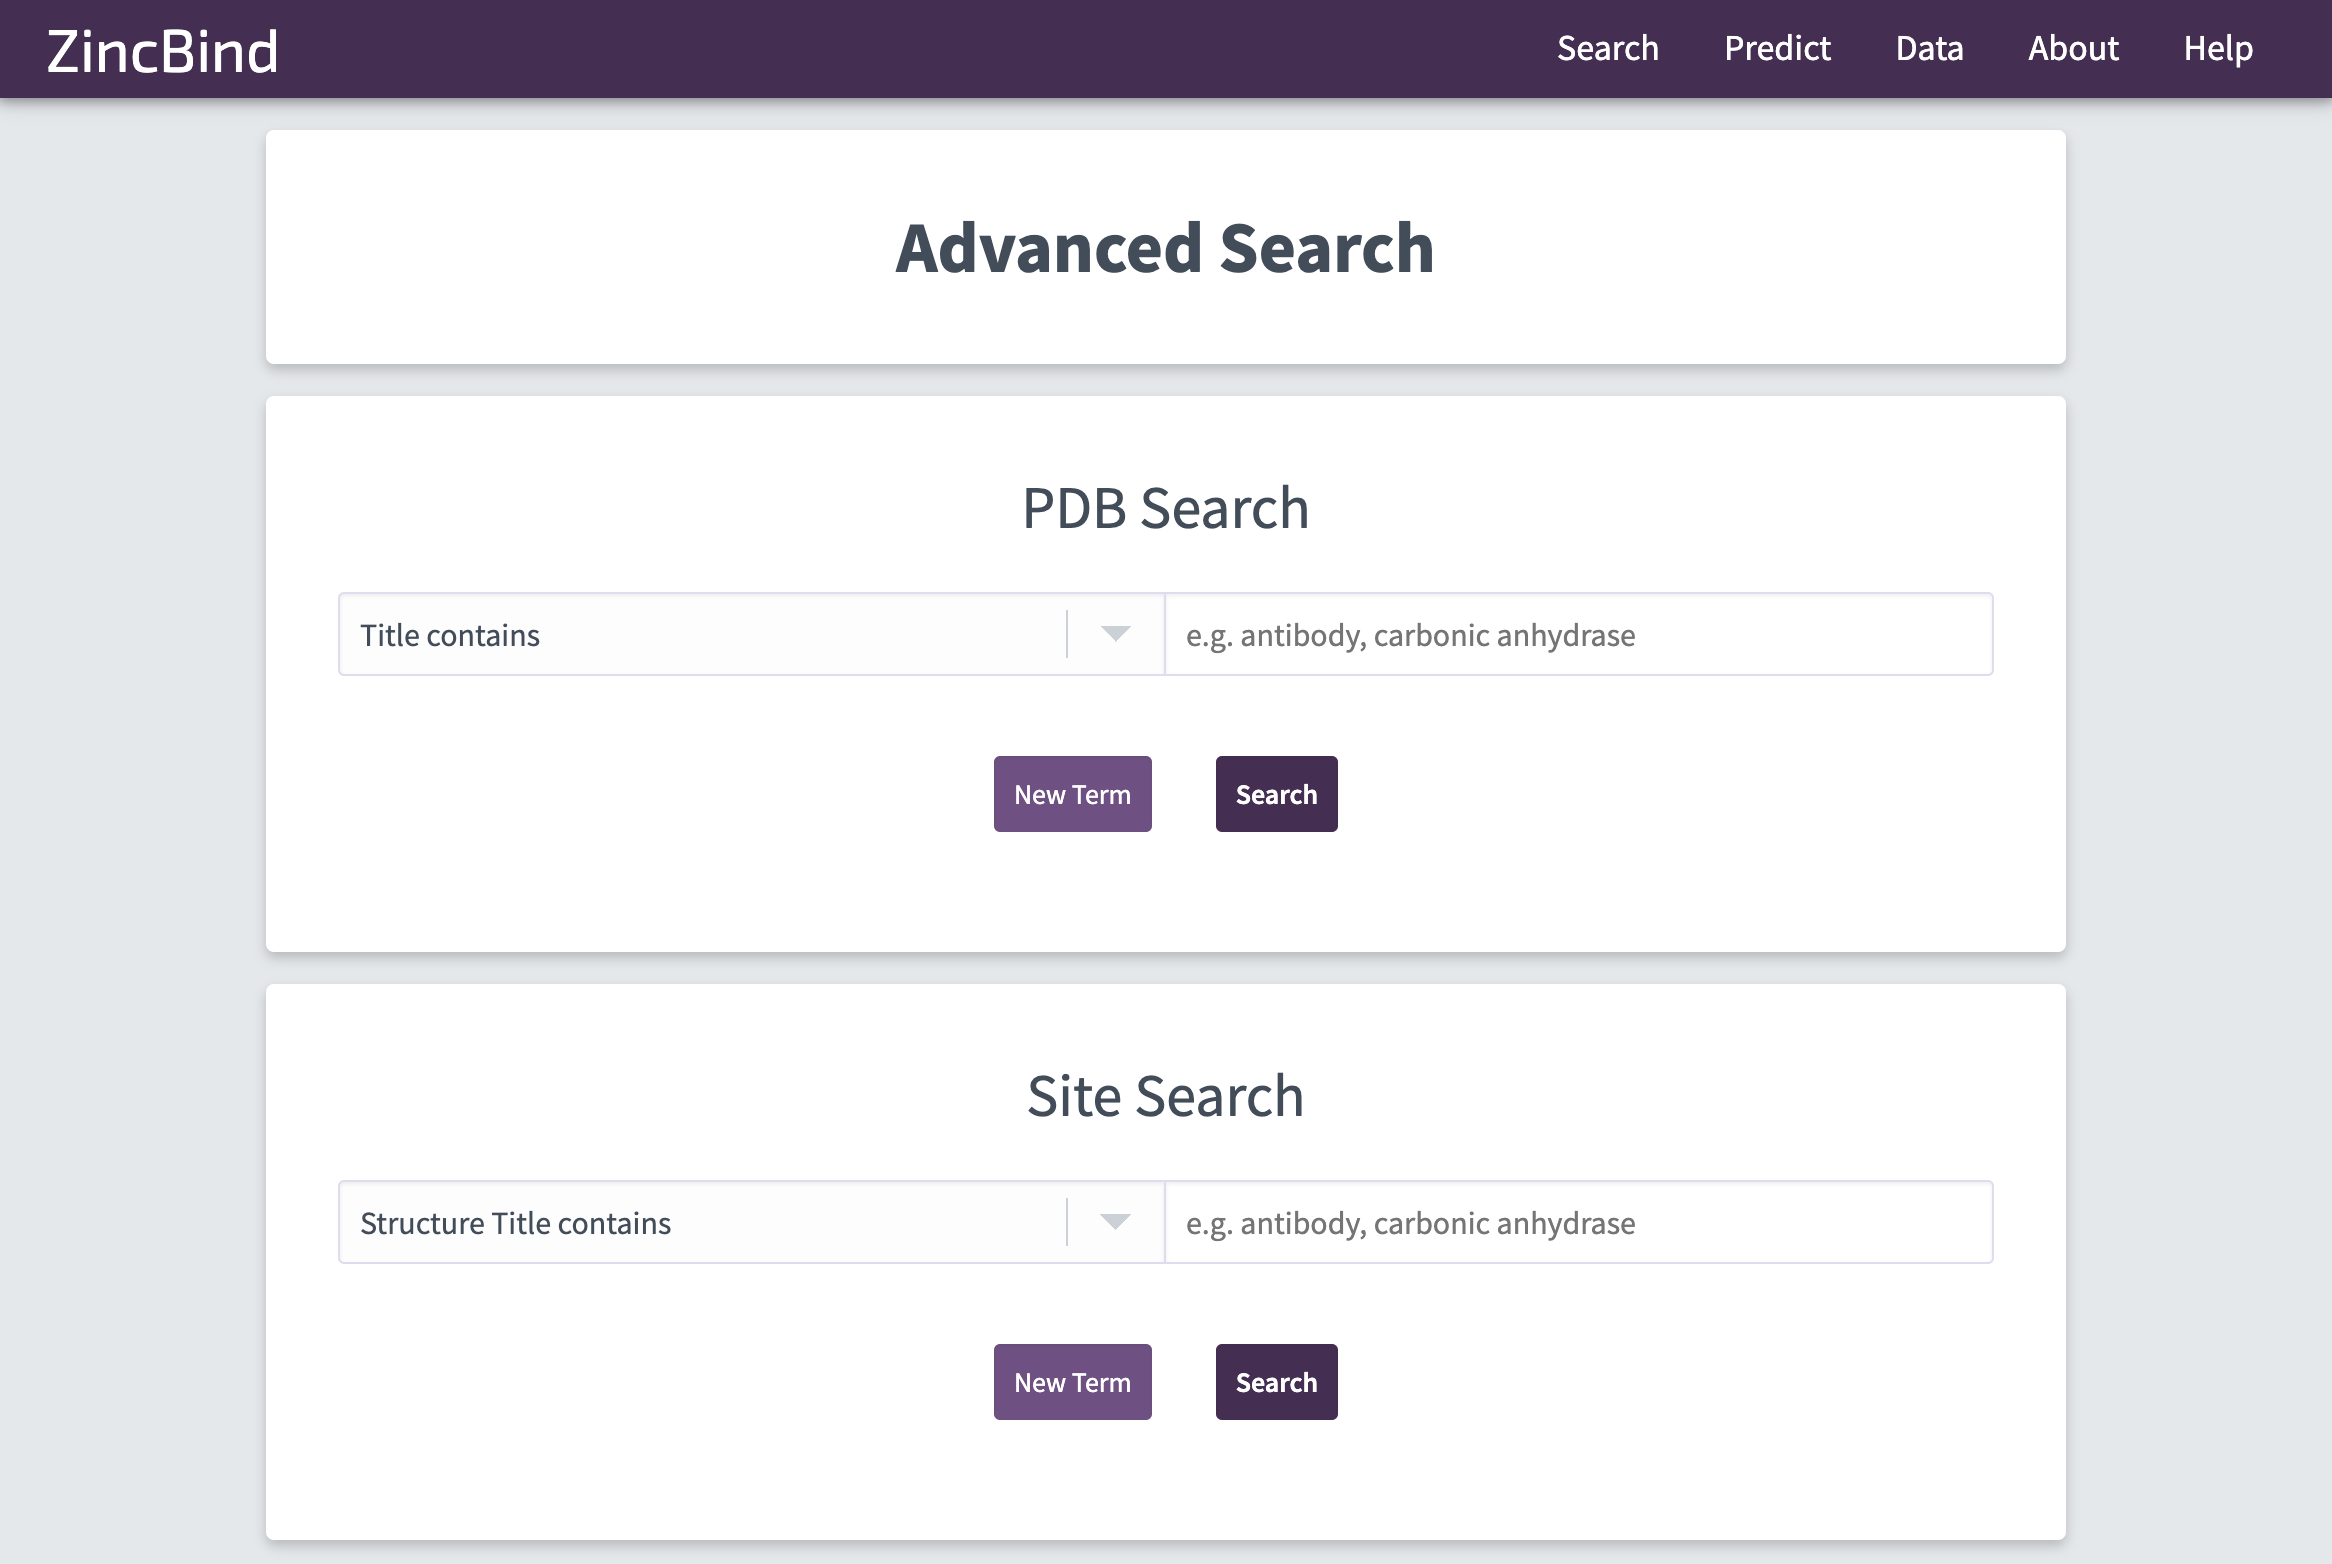
\includegraphics[width=1.0\textwidth]{Figures/zincbind-search.eps}
\caption[The advanced search interface.]{\label{fig:zincbind-search} The advanced search interface, allowing searching of
PDB files, or individual zinc binding sites.}
\end{figure}

Finally, the user can provide a sequence and perform a BLAST search against the database (see Figure~\ref{fig:zincbind-blast}). This uses the NCBI \texttt{blastp} binary on the backend, whose JSON output is processed by python functions and exposed via the GraphQL API. This produces chain sequence results (see Figure~\ref{fig:zincbind-blast-results}), rather than PDB/sites as the other methods do.

\begin{figure}
\centering
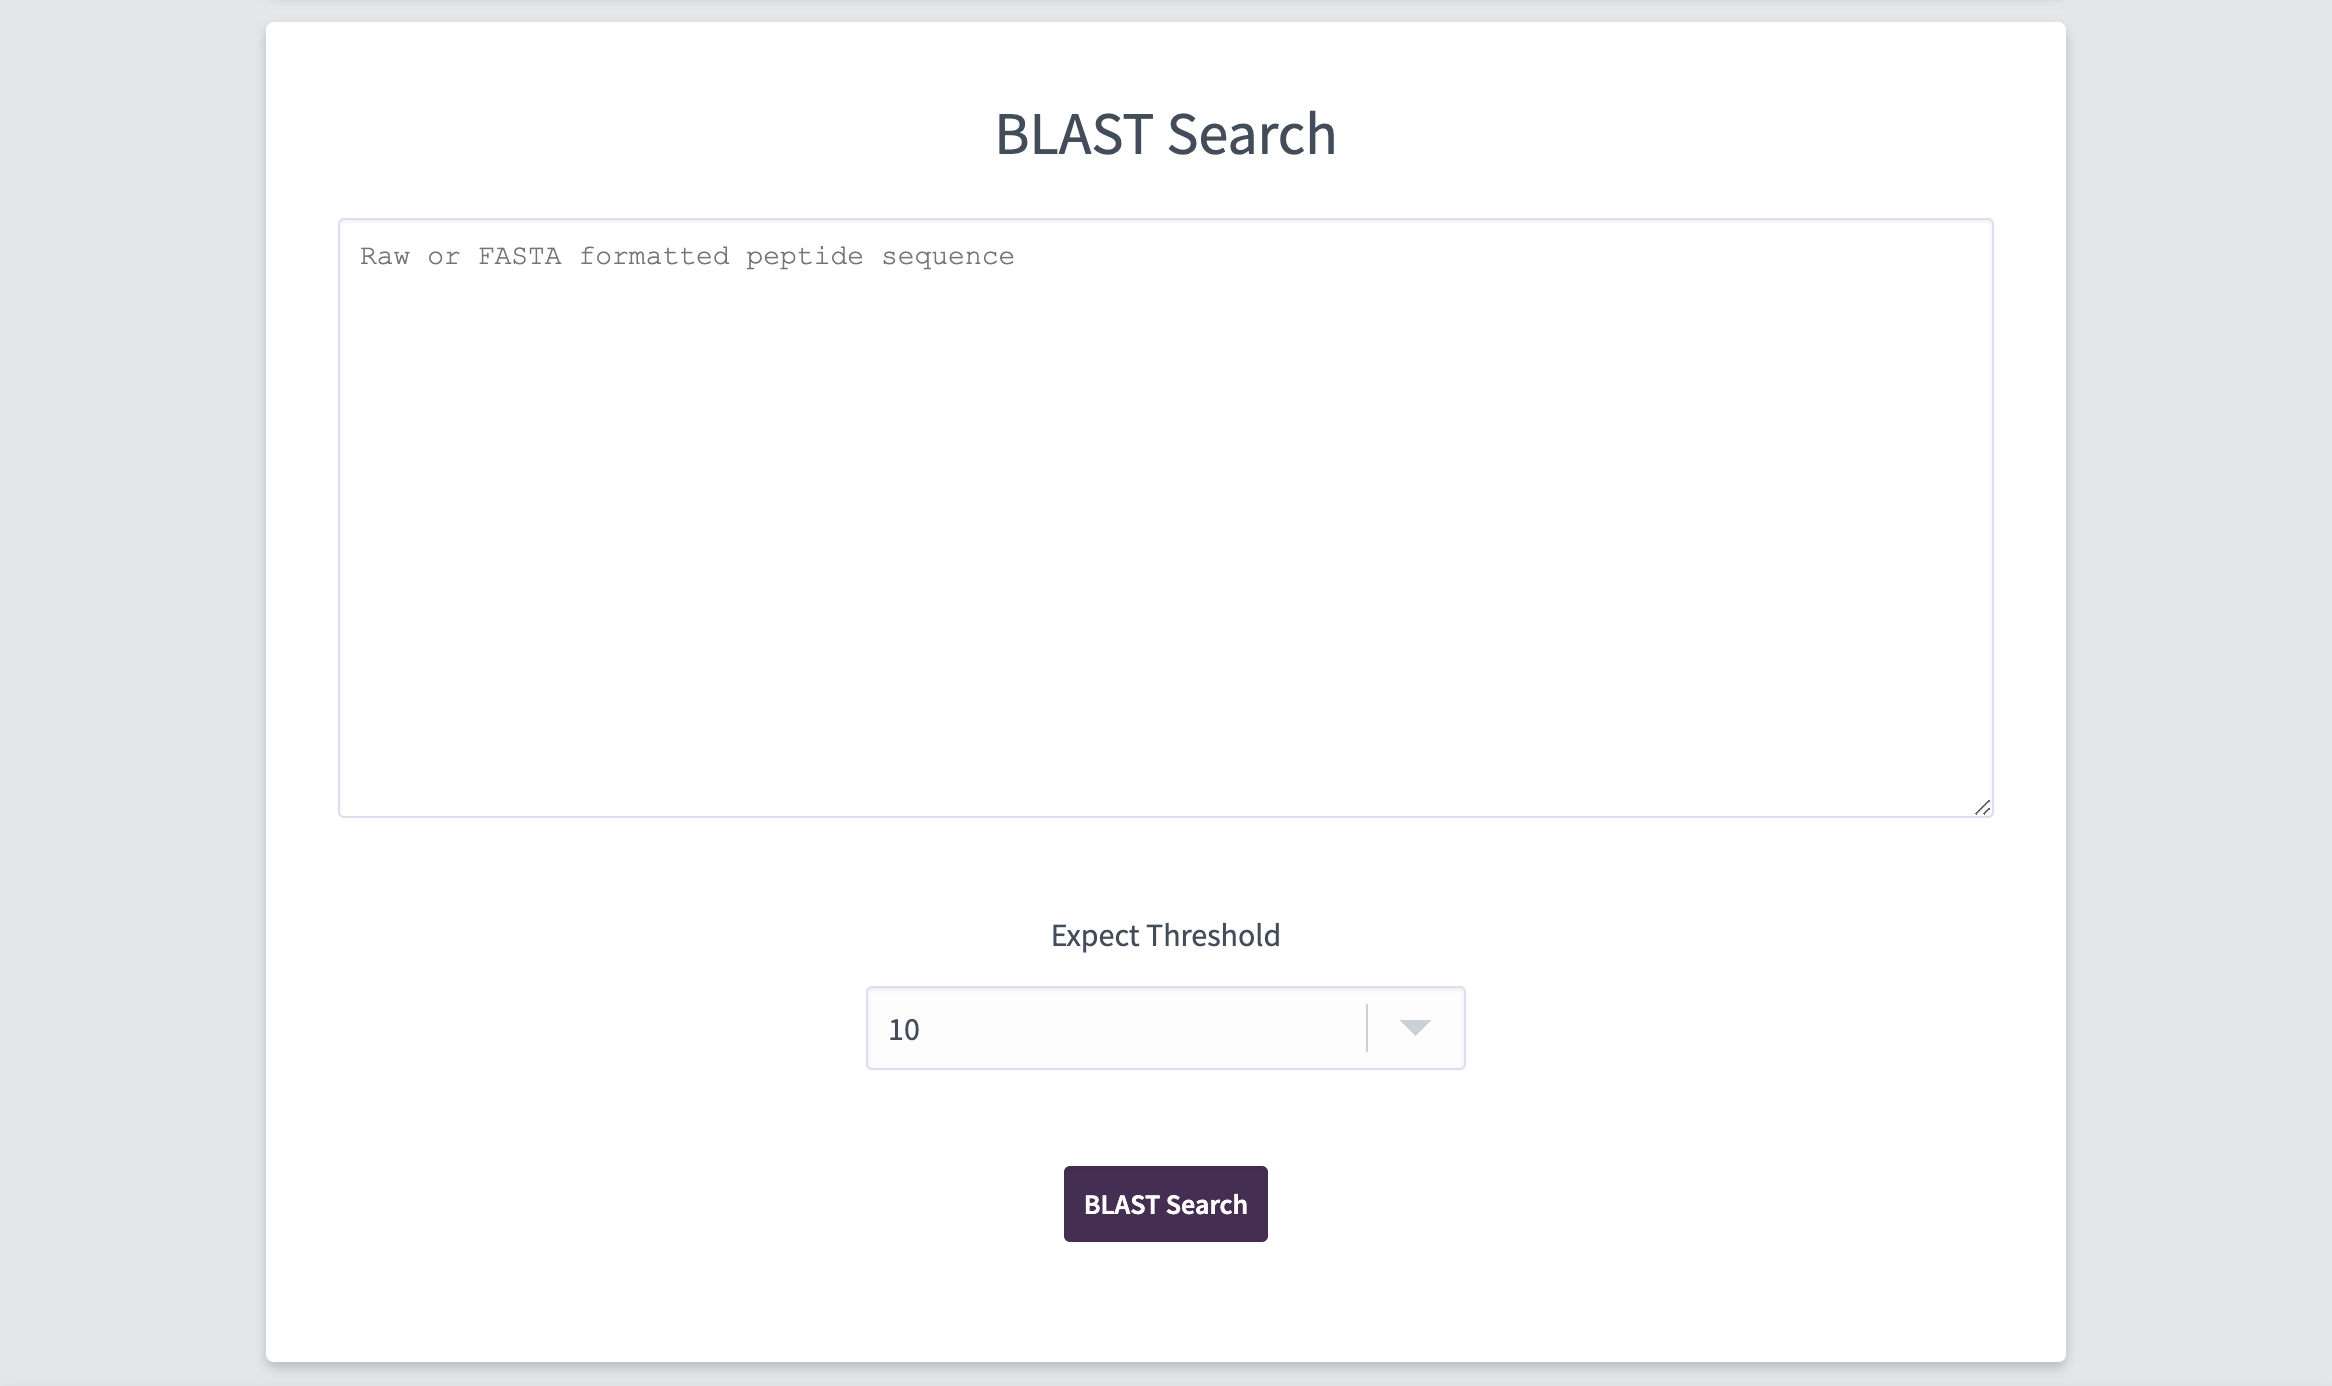
\includegraphics[width=1.0\textwidth]{Figures/zincbind-blast.eps}
\caption{\label{fig:zincbind-blast} The BLAST search interface.}
\end{figure}

The search results for the first two modes of searching are returned as a list of matching PDBs, with binding sites nested within them. Both the PDB and the sites themselves are clickable and will take the user to the page for that entity. Search results can be sorted by a variety of metrics, and are paginated to 25 results per page (see Figure~\ref{fig:zincbind-results}).

\begin{figure}
\centering
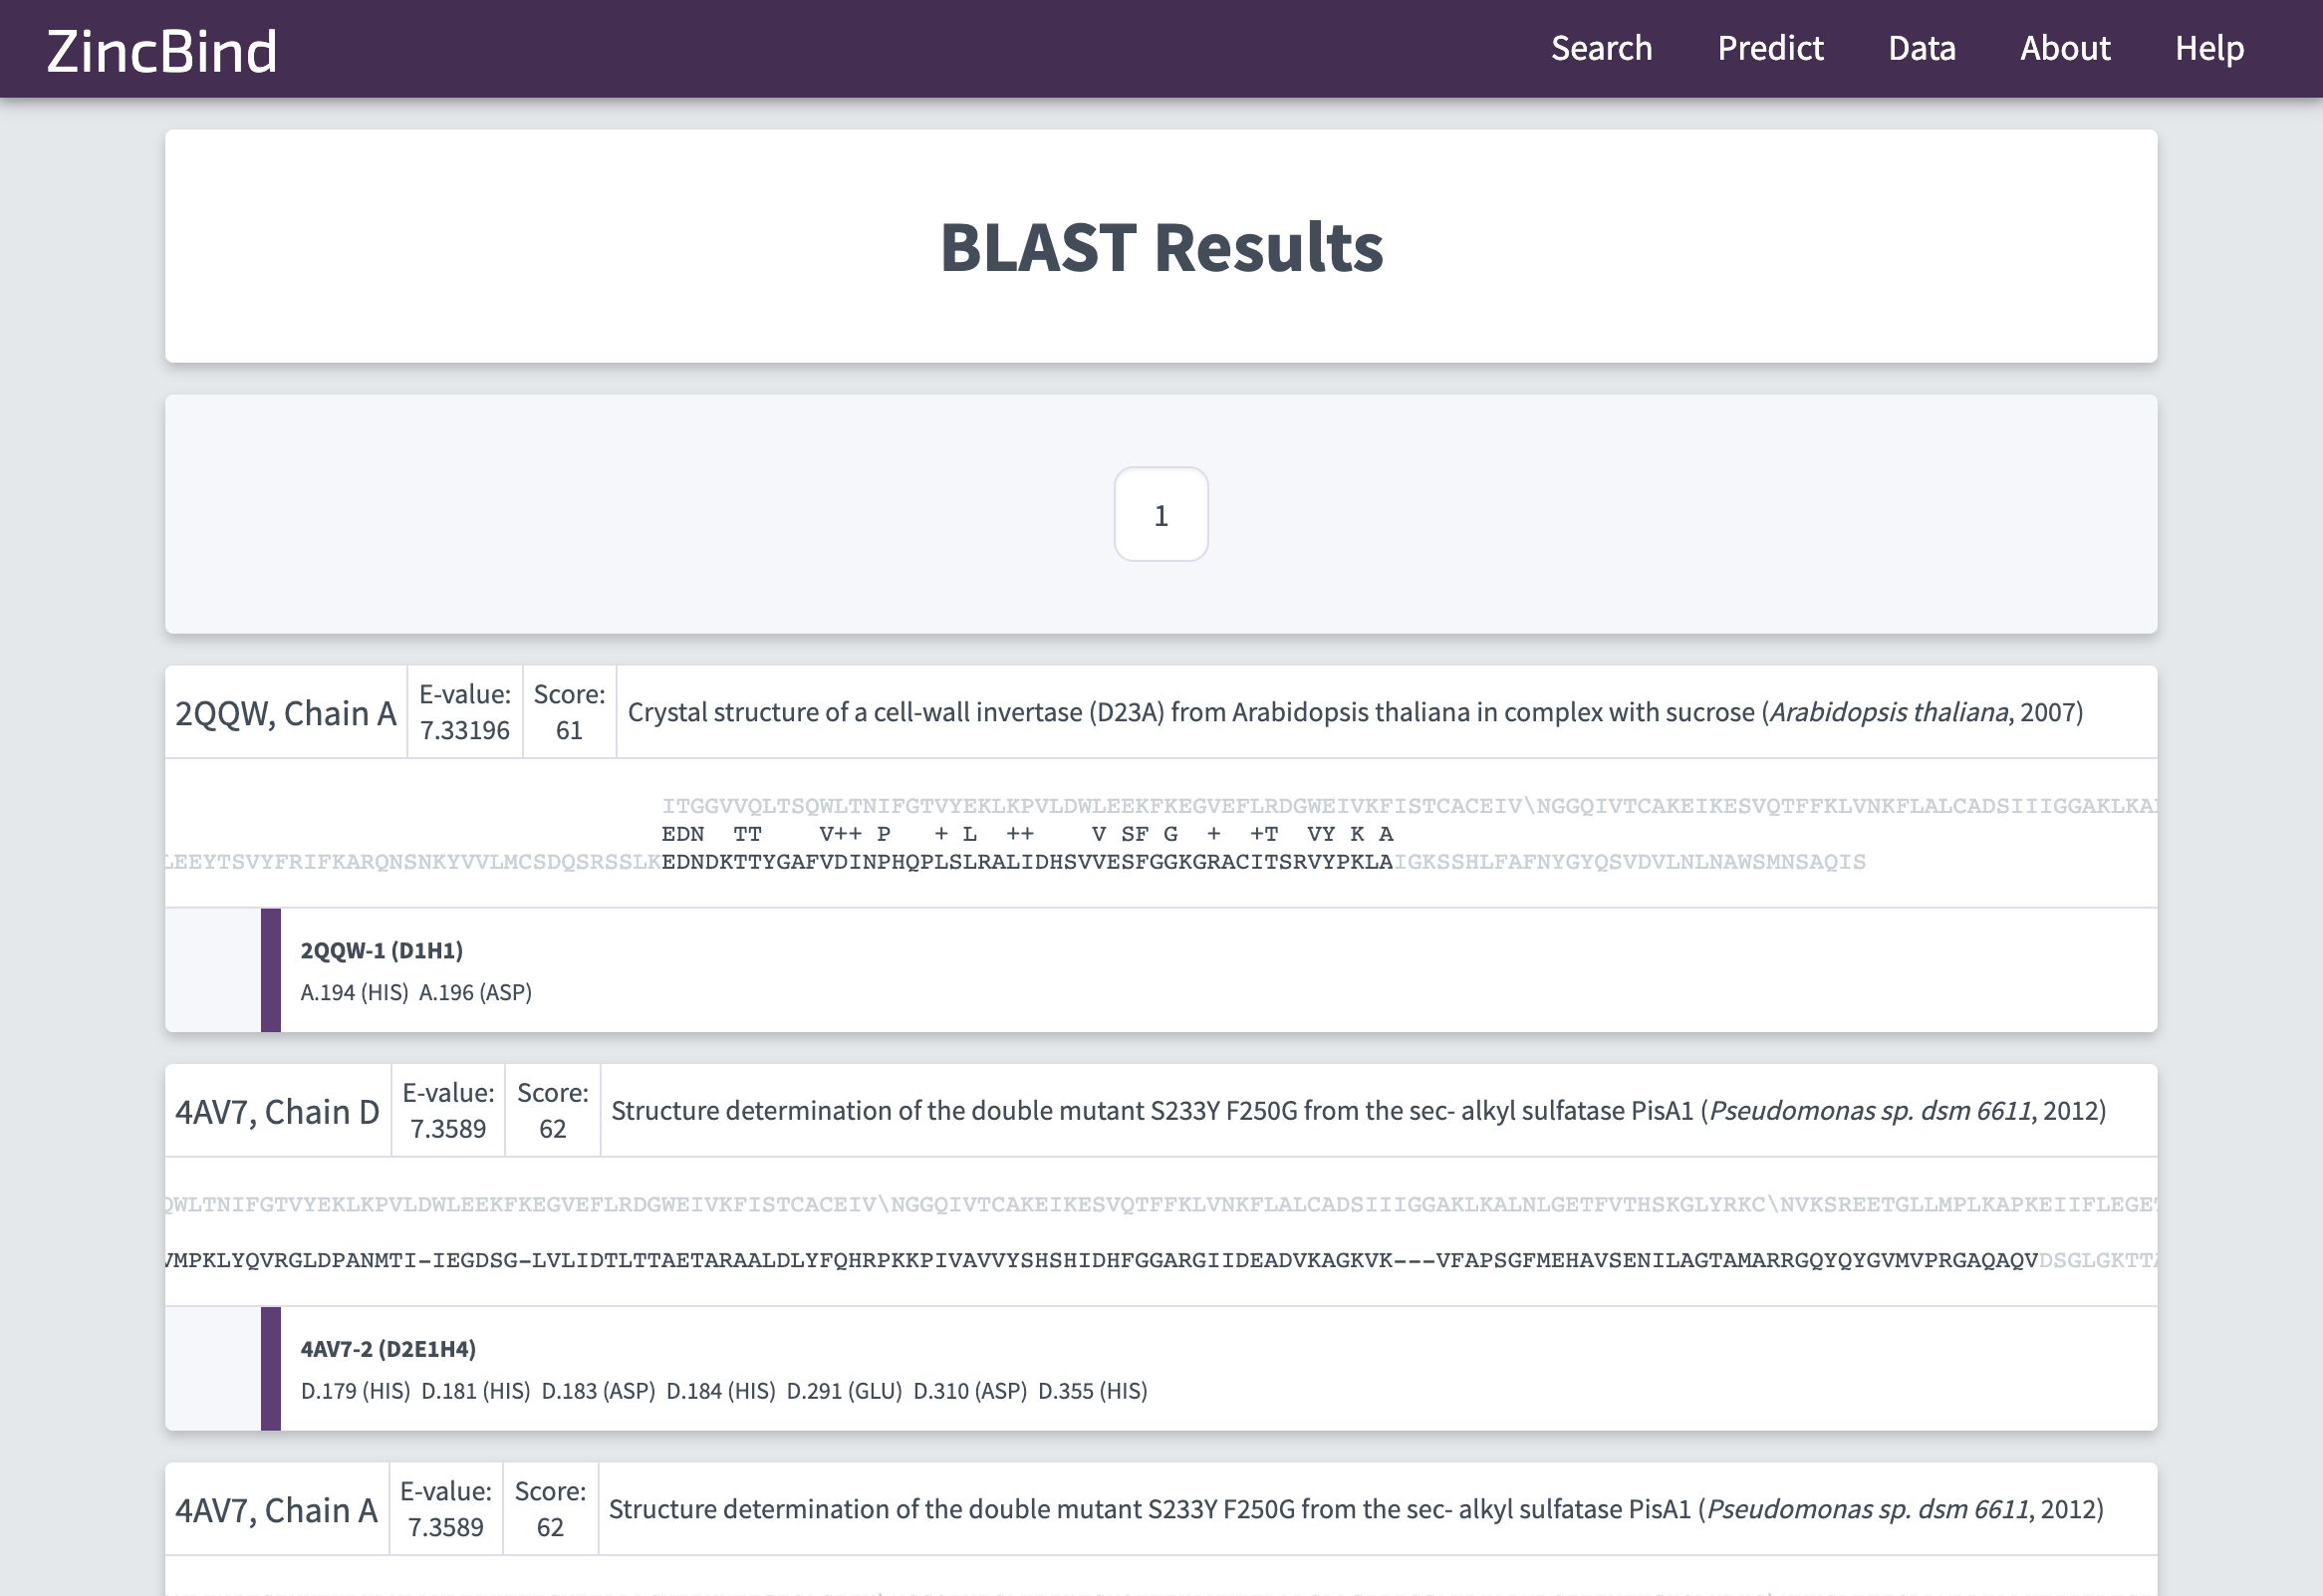
\includegraphics[width=1.0\textwidth]{Figures/zincbind-blast-results.eps}
\caption{\label{fig:zincbind-blast-results} An example of BLAST search results.}
\end{figure}

\begin{figure}
\centering
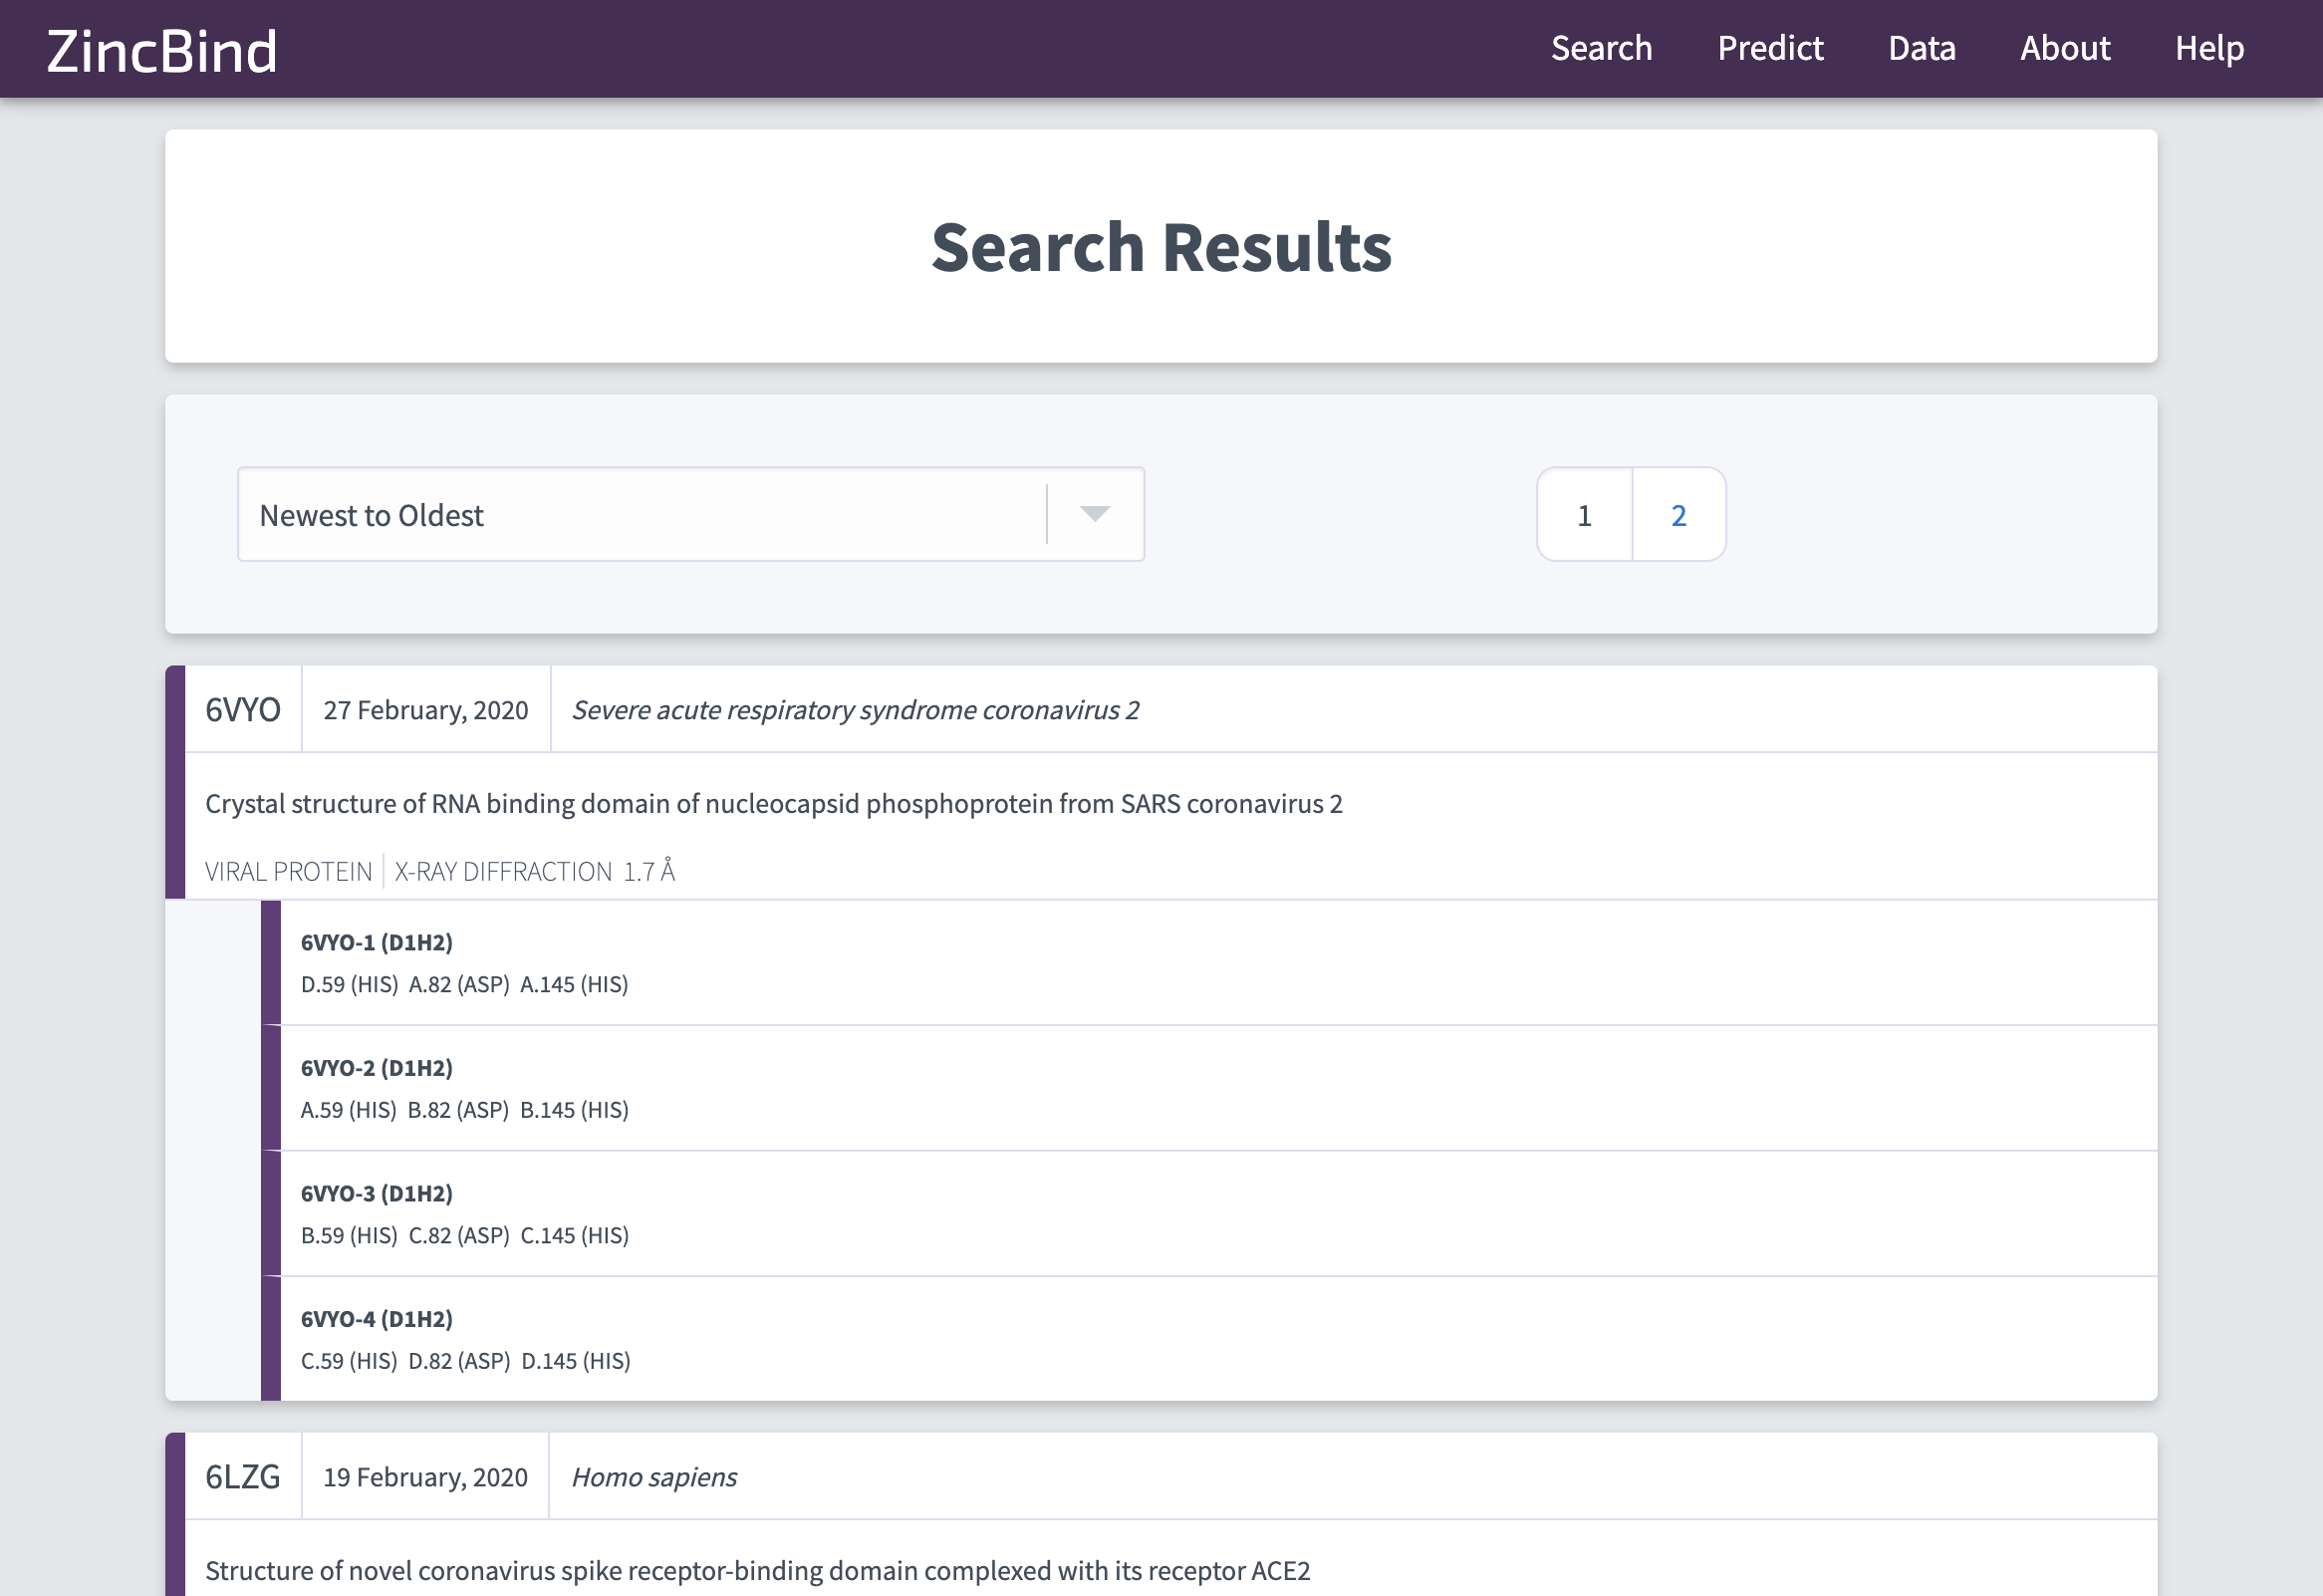
\includegraphics[width=1.0\textwidth]{Figures/zincbind-results.eps}
\caption[An example of paginated search results.]{\label{fig:zincbind-results} An example of paginated (over two pages
in this case) search result showing matching PDBs, and the zinc binding sites
they contain.}
\end{figure}

PDB pages represent PDB records (see Figure~\ref{fig:zincbind-pdb}). They provide basic information for that PDB (resolution, R-value, classification, source and expression organisms, experimental tehcnique, deposition date, and keywords --- the latter of which acts as a link to search by any of those keywords), as well as overviews of the zinc content of that PDB. The zincs associated with a binding site are listed as clickable links, while those without a binding site are listed along with their omission reason. Finally, there is a 3D manipulatable view of the PDB with all of its zinc binding sites. This uses the NGL Javascript library, and beside it is a set of basic options for manipiulating the view, such as rotation options, background colour, and binding site highlighting --- this is in addition to NGL's built-in touch/drag/zoom manipulation. Generally the PDB page limits itself to information relevant to the structure's role as a zinc binding protein, but a link to the equivalent RCSB page is also provided for more information.

\begin{figure}
\centering
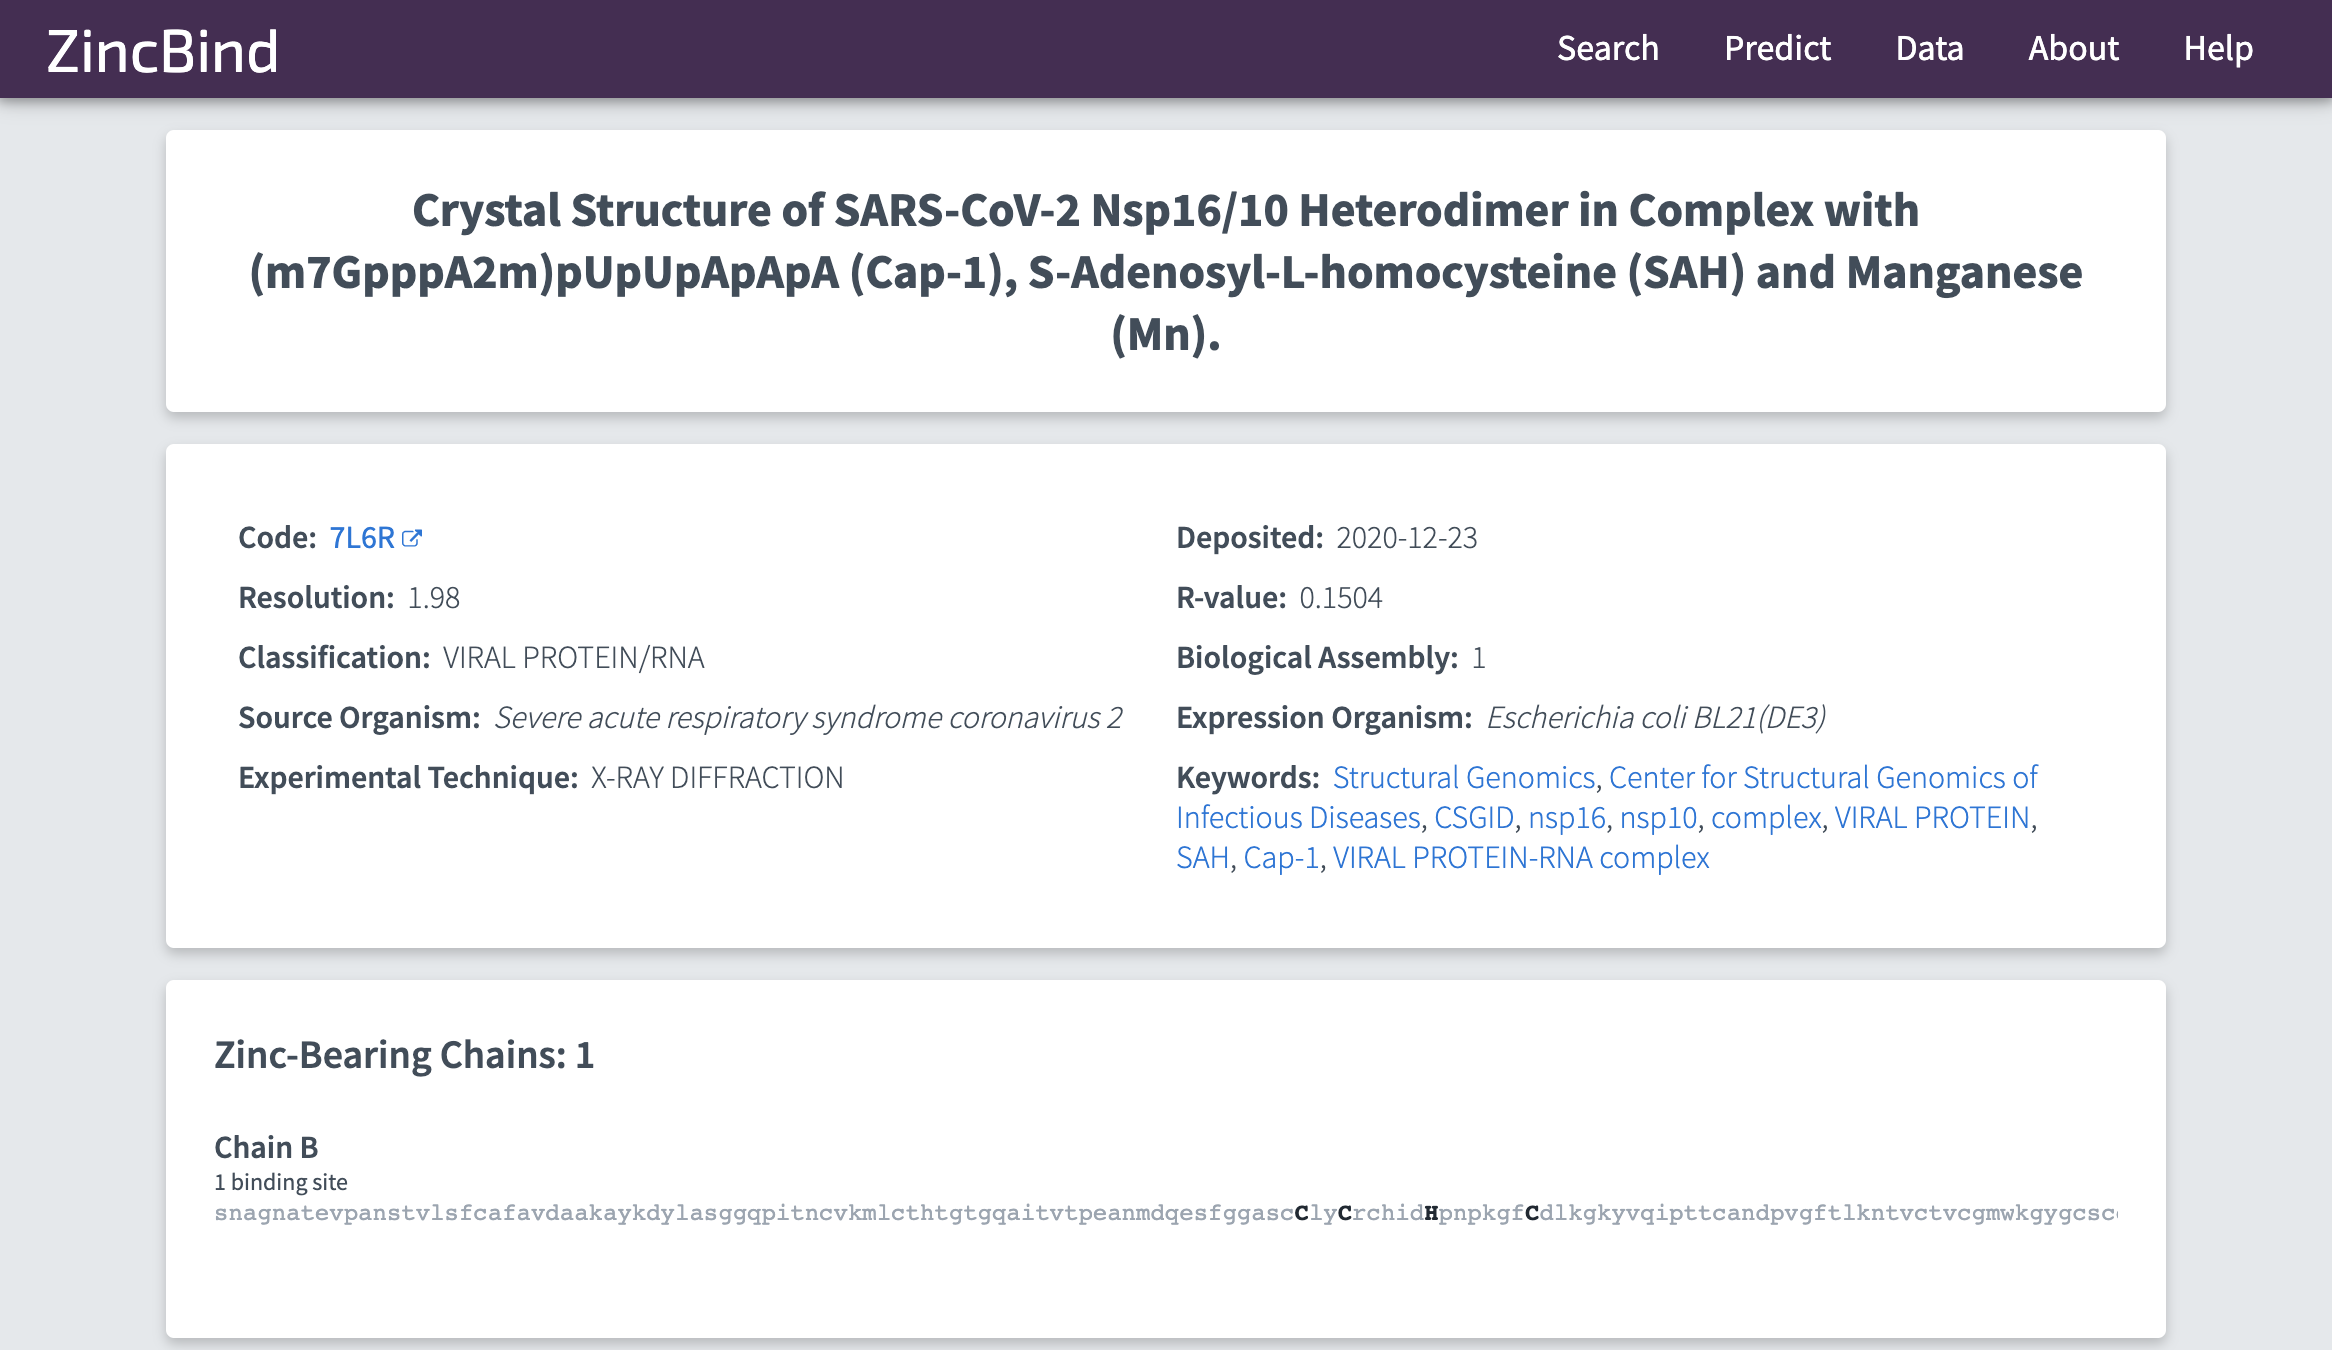
\includegraphics[width=1.0\textwidth]{Figures/zincbind-pdb.eps}
\caption{\label{fig:zincbind-pdb} An example of a PDB page in ZincBind, showing basic
information for that PDB. The three-dimensional structure view is further down the page.}
\end{figure}

The binding site pages (see Figure~\ref{fig:zincbind-site}) contain more detail for that specific binding site, such as its mode of coordination, and links to equivalent sites in the same group. There is also a 3D manipulatable model of the binding site on this page --- this is broadly the same as that on the PDB page, except zoomed in to the specific site and with selectable individual residues and metals. The page also contains a summary of information for the containing PDB, and a link to that PDB's page.

\begin{figure}
\centering
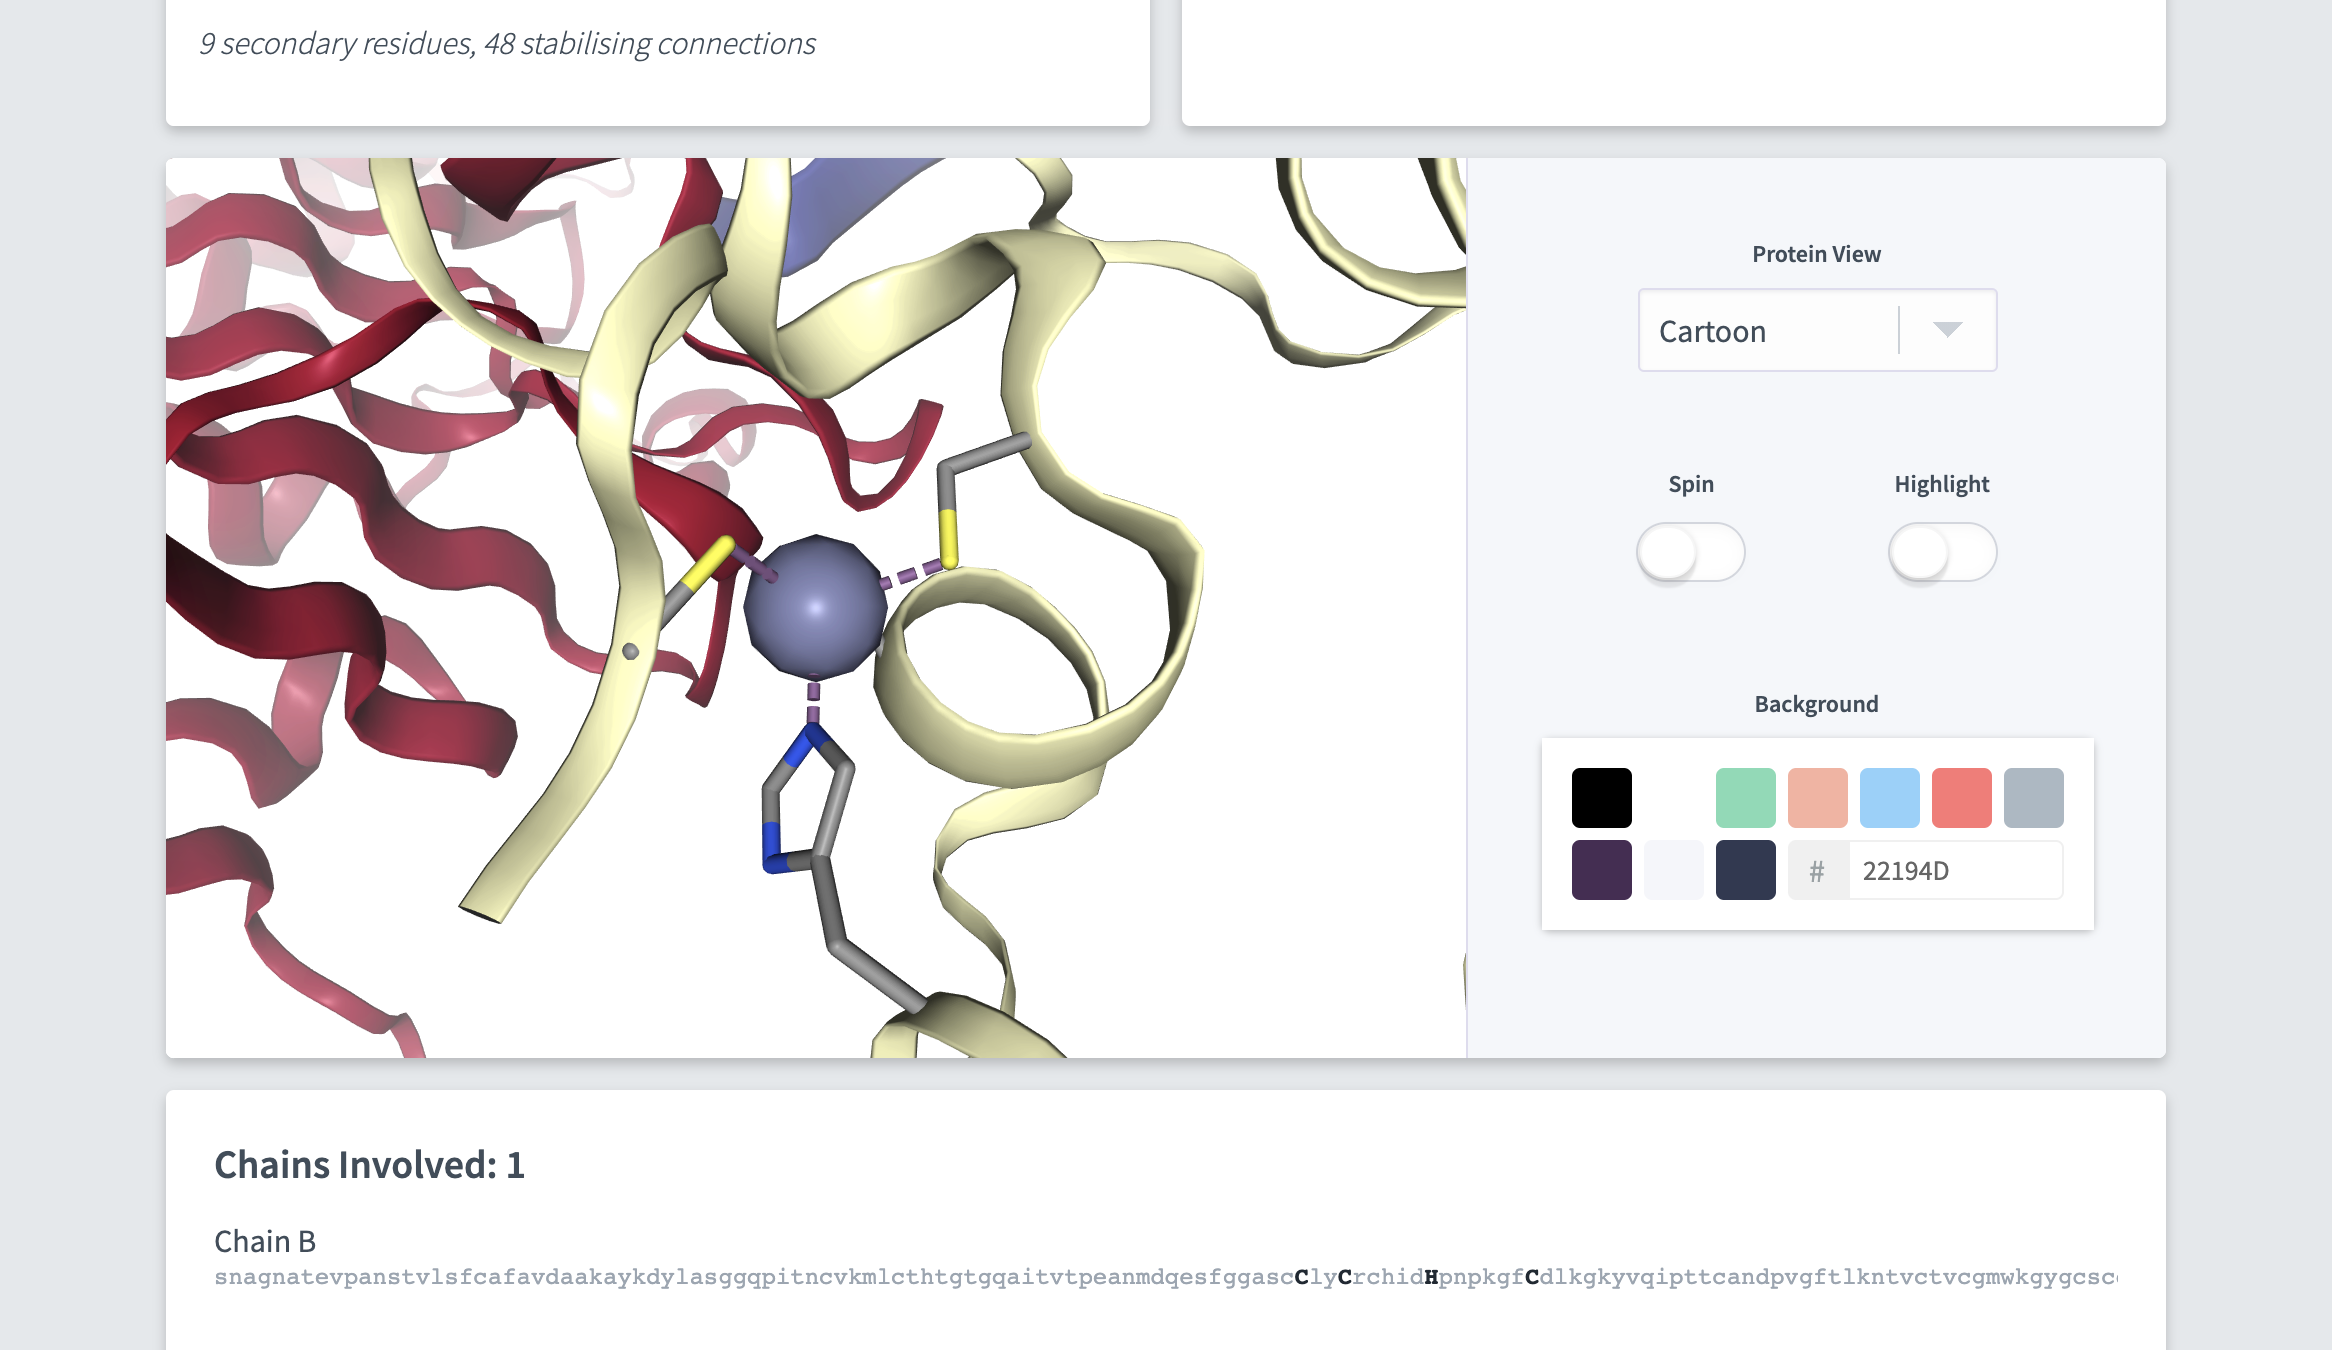
\includegraphics[width=1.0\textwidth]{Figures/zincbind-site.eps}
\caption[An example of a binding site page in ZincBind.]{\label{fig:zincbind-site} An example of a binding site page in ZincBind, with the manipulatable
3D NGL viewer, zoomed in to this binding site.}
\end{figure}

ZincBind also has a page that gives an overview of the dataset as a whole (see Figure~\ref{fig:zincbind-data}). This contains charts for residue distribution, experimental methods, residue codes, resolution, species frequency, and PDB classification. These are intended to give a sense of the key properties of the database `at a glance'. There are also links to a page containing all data (essentially a modified version of the search results page that shows all PDBs, paginated), a link to an overview of the GraphQL API, and a link to a page showing how the sites are clustered into families and groups. Here each group lists the keywords and classifications that the sites in that group have in common to try to provide an automated way of annotating what the binding site the group represents actually does (see Figure~\ref{fig:zincbind-group}).

\begin{figure}
\centering
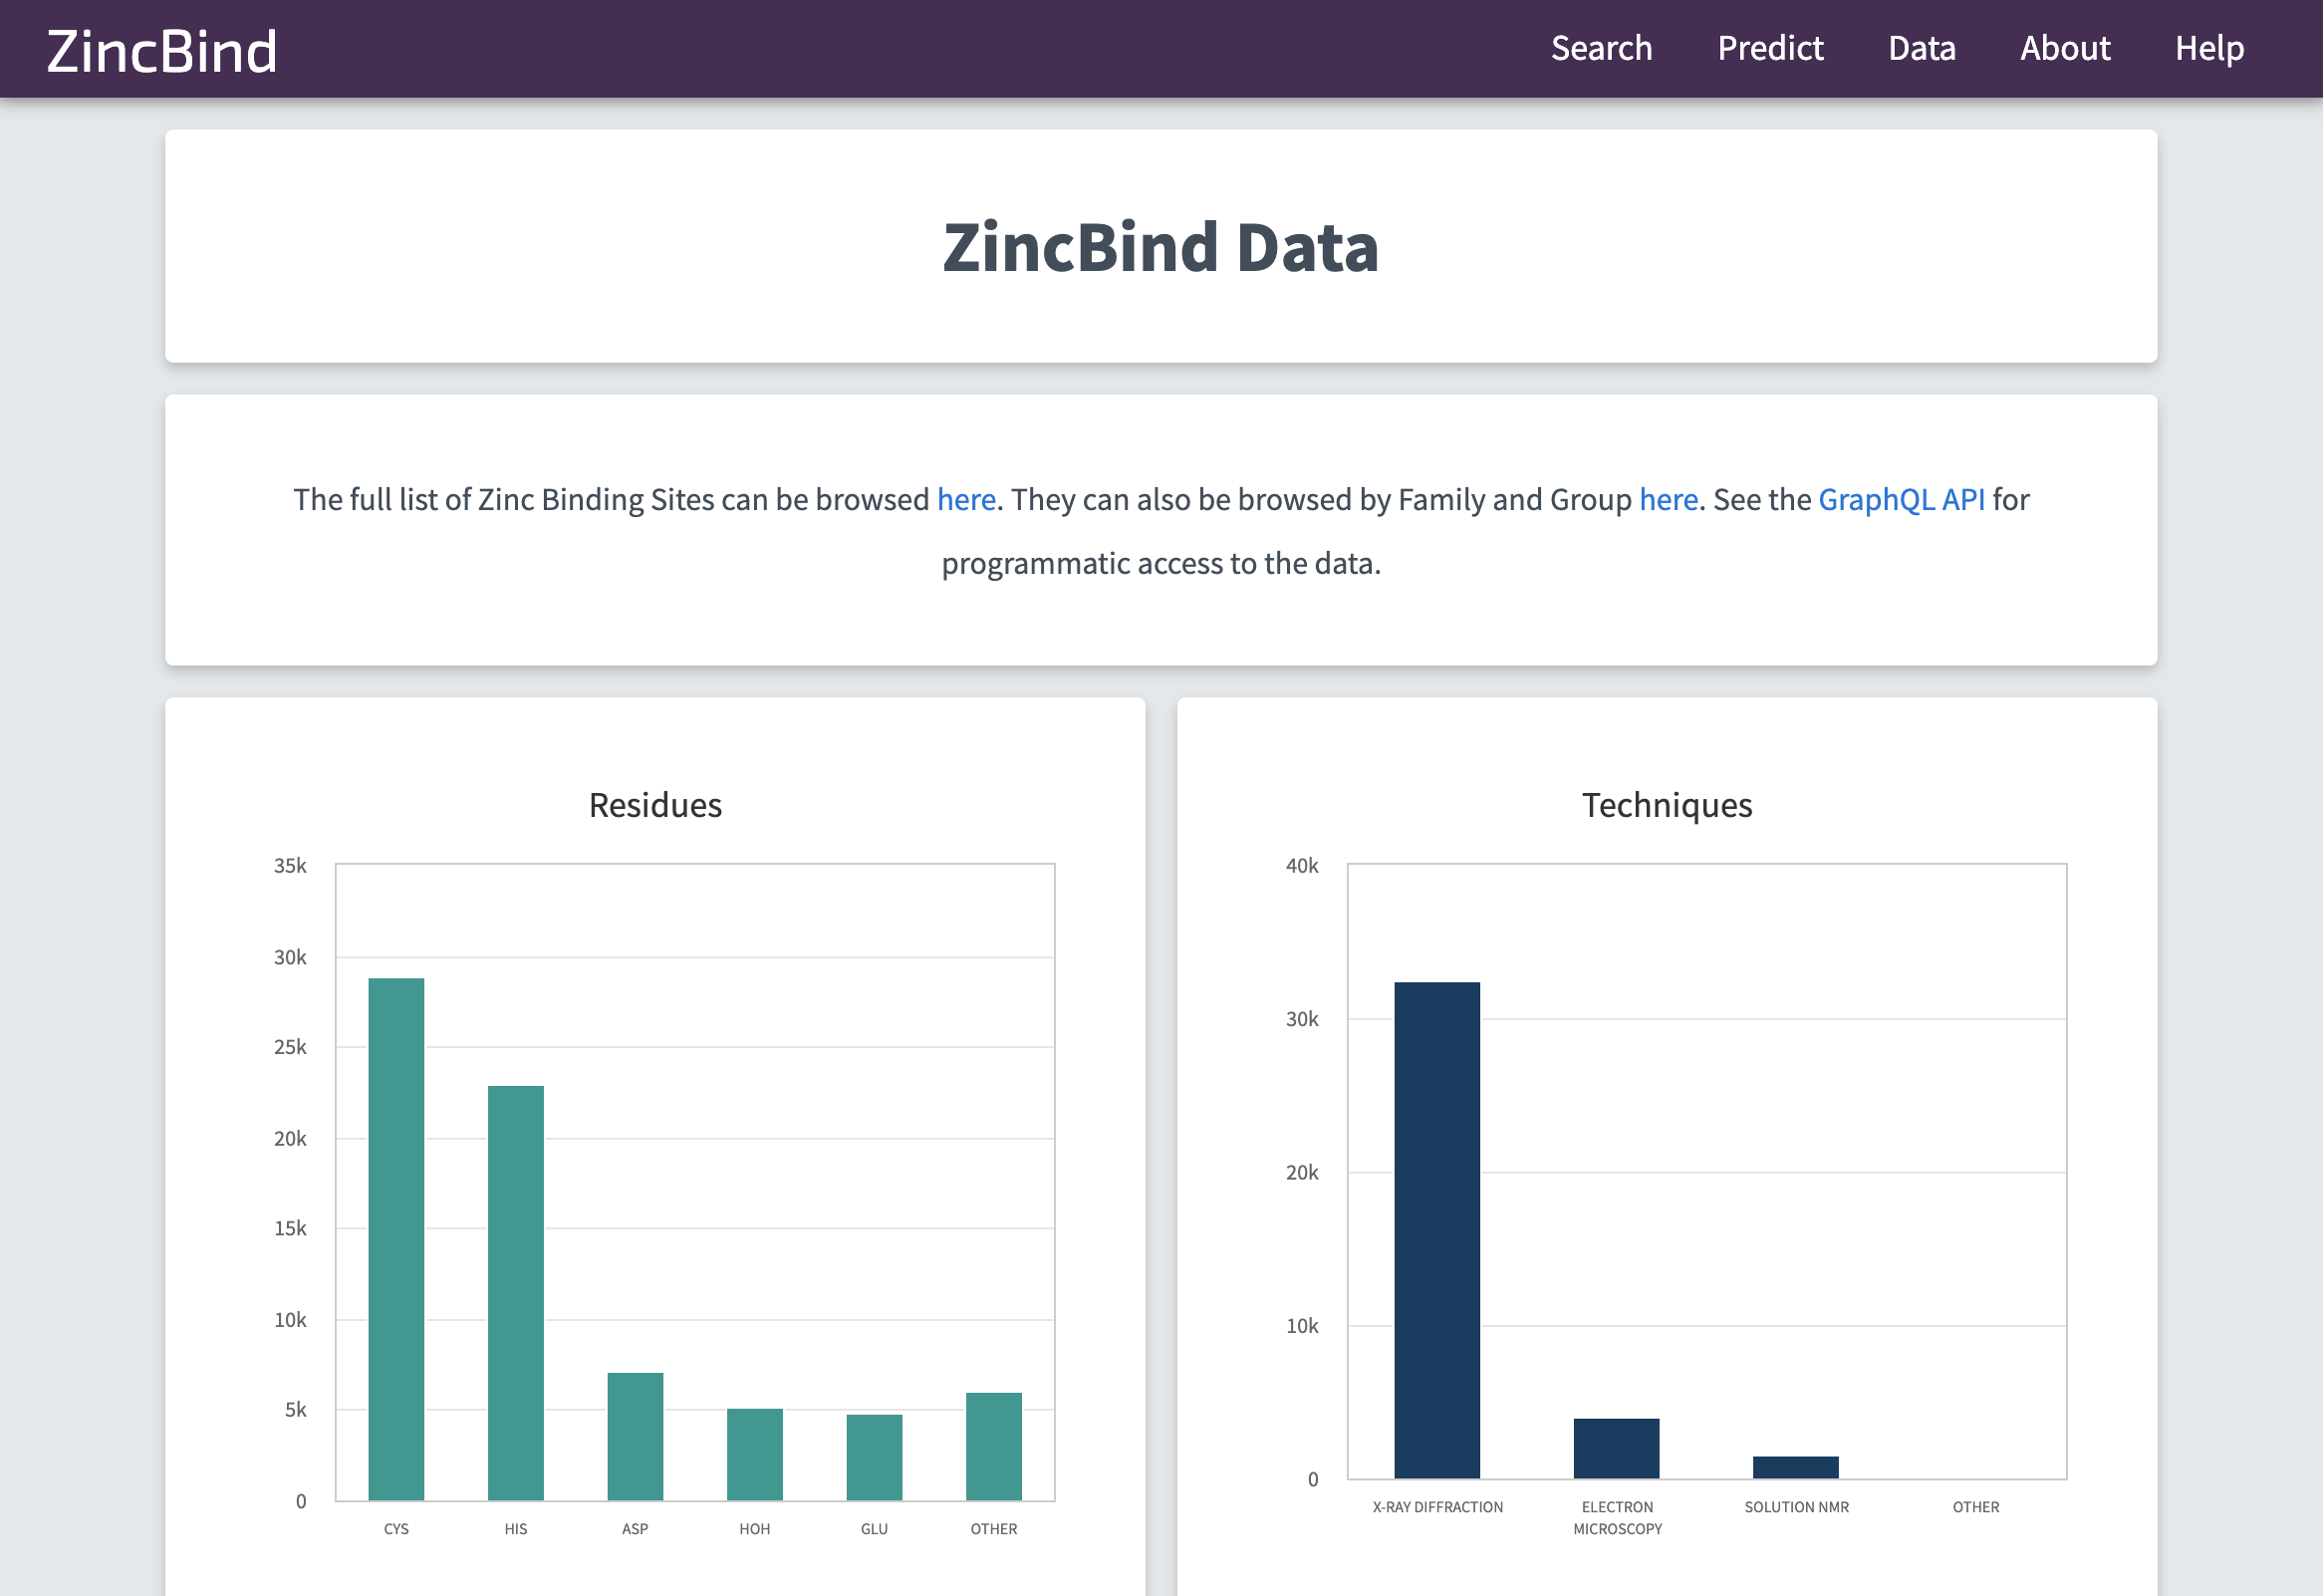
\includegraphics[width=1.0\textwidth]{Figures/zincbind-data.eps}
\caption{\label{fig:zincbind-data} Overview statistics for the dataset presented on
the ZincBind data page.}
\end{figure}

\begin{figure}
\centering
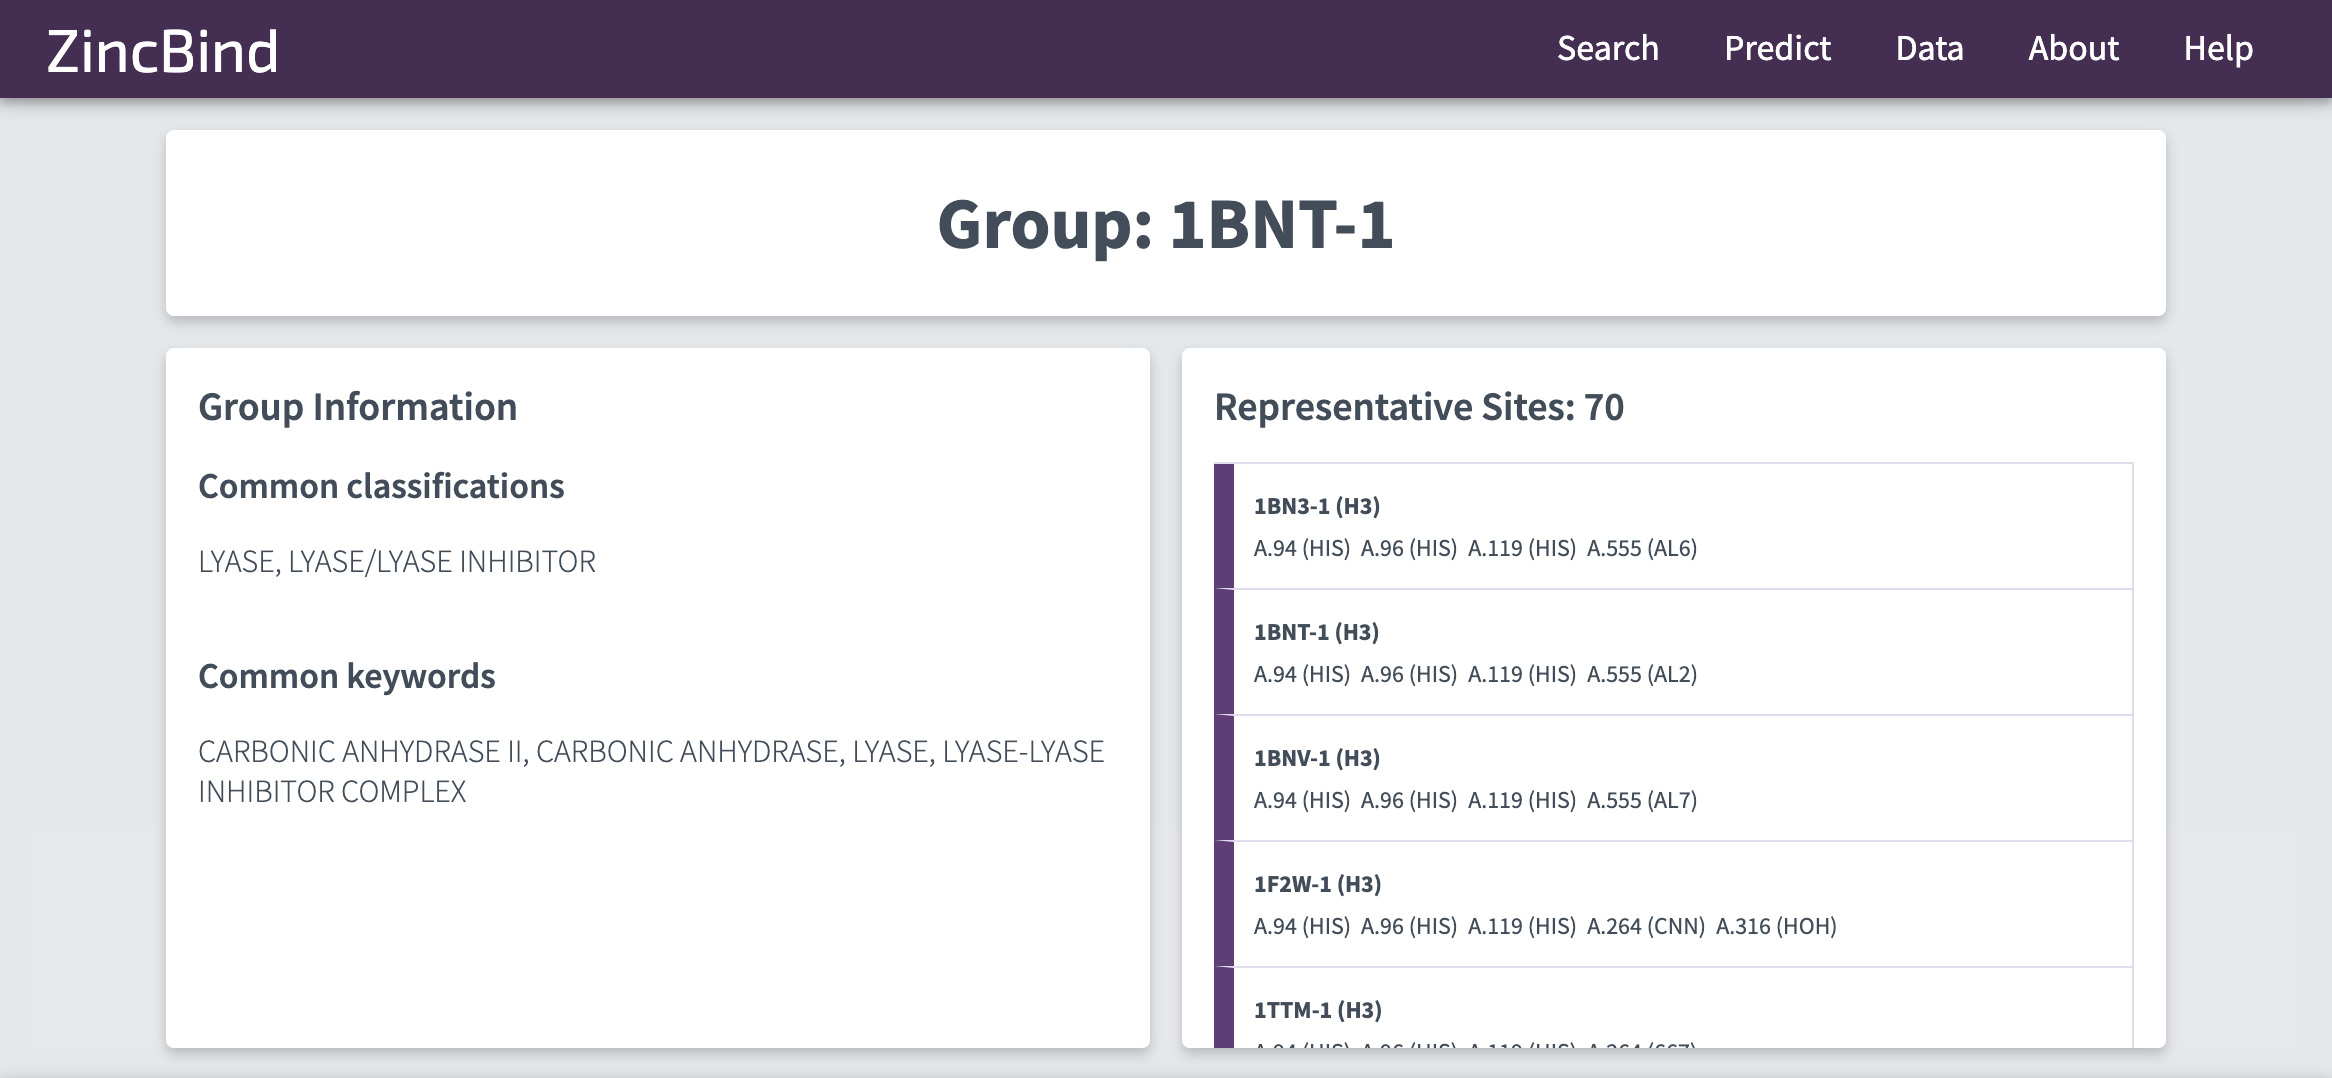
\includegraphics[width=1.0\textwidth]{Figures/zincbind-group.eps}
\caption{\label{fig:zincbind-group} A ZincBind group page, summarising the clustered zinc
binding sites and providing links to individual site pages.}
\end{figure}

There is a page dedicated to the prediction of binding sites that uses the separate prediction API, but this will be covered in greater detail in the next chapter.

Finally, ZincBind has a help page, structured as a series of questions that a user may have.

Ultimately, the website is intended to serve as a way of broadening access to the database, which is continually updated. The API provides access to the data for researchers who need bulk access to the data, whereas the web frontend allows an individual to explore the data more casually to get a sense of what research might be carried out with it.

\section{Data Analysis}

The finished dataset offers a useful insight into the general properties of zinc binding sites, or at least that subset of zinc binding sites for which structural information is available. Some of these properties are of use in building predictive models of zinc binding sites, whereas others are of more general interest. An overview of the main findings that can be gleaned from the dataset will be presented here. All values are correct at the time of writing (February 2021), though as this is a continually and automatically updated dataset, the precise values will vary as time goes on. It is not anticipated that these changes will alter the overall conclusions, as the dataset is very large already.

\subsection{The Prevalence of Zinc}

Of the 174,014 PDB structures in the Protein Data Bank at the time of the most recent database update, 17,556 contained at least one zinc atom and are accounted for in ZincBind. This proportion, 10.1\%, is very close to the 10\% of human proteins usually said to contain zinc, though as the Protein Data Bank does not purport to be a representative sampling of any genome, human or otherwise, there was no particular reason for this to be the case.

\subsection{Qualifying Atoms}

In total, when run in Fenruary 2021, ZincBind identified 65,595 zinc atoms and 1,138 other metal atoms associated with zinc atoms when searching the raw coordinates of the PDB asymmetric units. Other metals are only stored in ZincBind if they are part of a multi-metal binding site with at least one zinc atom, so the vast majority of metals in the database are zinc. Of the non-zinc metals, the most common of these `co-active' metals are magnesium, potassium, iron and copper (see Table~\ref{tab:metalcount}).

\begin{table}
  \caption{\label{tab:metalcount}Prevalence of various non-zinc metals in ZincBind.}
\begin{center}
\begin{tabular}{lll} \hline
Metal & Count & Relative Percentage  \\ \hline
Potassium & 319   & 28.0\% \\
Iron      & 188   & 16.5\% \\
Copper    & 15    & 13.6\% \\
Magnesium & 132   & 11.6\% \\
Sodium    & 100   & 8.8\%  \\ 
Calcium   & 90    & 7.9\%  \\
Manganese & 75    & 6.6\%  \\
Cadmium   & 38    & 3.3\%  \\
Cobalt    & 31    & 2.7\%  \\
Nickel    & 6     & 0.5\%  \\
Vanadium  & 3     & 0.3\%  \\
Barium    & 1     & 0.1\%  \\ \hline
\end{tabular}
\end{center}
\end{table}

Of the 65,595 zinc atoms in the database, 24,246 (37.0\%) are not associated with any binding site, and are in the database solely to acknowledge their existence. The most common reason for not assigning a zinc atom to a binding site is that the atom is duplicated multiple times in the asymmetric unit, but appears only once in the biological assembly used for processing; 13,124 metals were excluded for this reason. For example, PDB entry 1A4L contains four chains, each with one zinc atom, but the biological assembly only uses one. The other three are stored in ZincBind with an omission reason, but have no binding site assigned to them. Figure~\ref{fig:omission} shows the breakdown of zinc atoms by omission reason.

Using the full biological assembly leads to zinc ions being both excluded, and included as being associated with binding sites. As stated above, it is common for the asymmetric unit of a PDB file to contain multiple copies of the biomolecule of interest as a result of crystallization, but once the `correct' assembly is chosen, these duplicated zinc atoms will be absent from the final structure. Conversely, using the full biological assembly rather than just the raw asymmetric unit coordinates of the PDB is crucial when the zinc atom is present at an interface between chains. In the asymmetric unit, there may be a single residue coordinating with the ion; if symmetry were not considered, such a model would be discarded by the ZincBind algorithm as a salt.

\begin{figure}
\centering
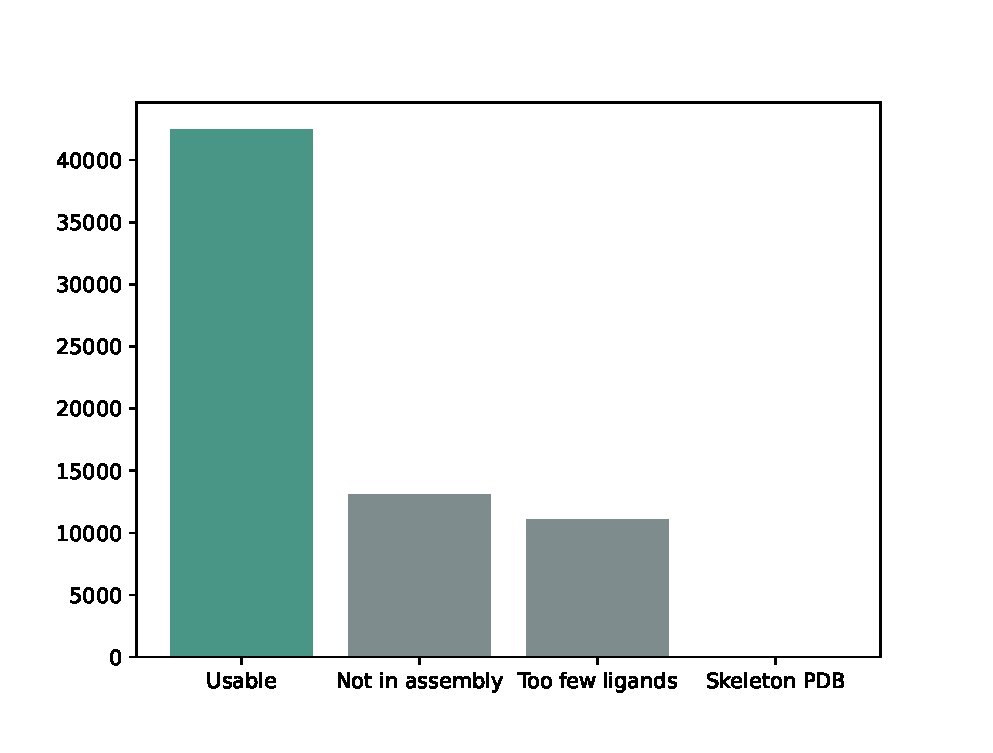
\includegraphics[width=1.0\textwidth]{Figures/omission.eps}
\caption[The relative frequency of omission reasons for zinc
atoms that were ultimately not assigned to a binding site.]{\label{fig:omission} Illustrating the relative frequency of omission reasons for zinc
atoms that were ultimately not assigned to a binding site. There were 8 which were omitted because
the PDB structure did not contain side chains --- insignificant compared with the other two reasons.}
\end{figure}

\subsection{Zinc Binding Sites with High Representation}

The 42,487 metal atoms, for which binding site information is stored, are part of a total of 38,035 zinc binding sites in ZincBind. After clustering the proteins at 90\% sequence identity and then clustering the binding sites as described above, there are 17,471 unique zinc binding sites in the database. The binding site with the most copies is from carbonic anhydrase (355 copies), a catalytic serum protein and, as already noted, the first known zinc binding protein. This is followed by JMJD2D (247 copies), a lysine-specific demethylase. 11,785 (67.5\%) zinc binding sites are currently unique in that they have only one structure, and are therefore only represented once in ZincBind. This distribution is shown in Figure~\ref{fig:group-clusters}

\begin{figure}
\centering
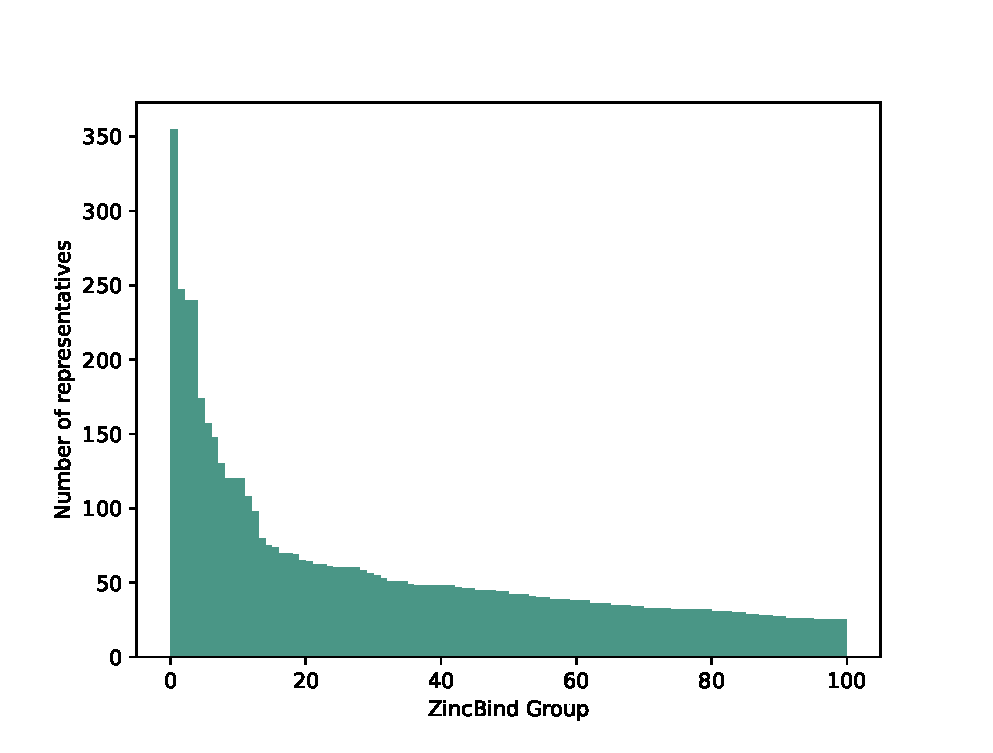
\includegraphics[width=1.0\textwidth]{Figures/group-clusters.eps}
\caption{\label{fig:group-clusters} The distribution of binding sites among groups for the hundred most populated groups.}
\end{figure}

For each cluster of equivalent zinc binding sites, the best-resolution structure is chosen to provide a single site which is flagged as the `representative' for that cluster.

\subsection{Liganding Residues}

The binding residues that dominate zinc binding sites are well established: cysteine, histidine, and the acidic residues aspartate and glutamate. This is supported by the data in ZincBind. There are a total of 161,324 liganding residues in ZincBind, of which those four residue types, together with water, comprise 93.0\% of all zinc-liganding residues. Note, however, that this considers every binding site in the database. When non-redundant sites are studied (i.e.\ only one site per cluster thereby removing the bias towards more intensely studied proteins), these five comprise a slightly smaller percentage of zinc-liganding residues (92.0\%). This suggests that the binding sites most frequently appearing in the PDB show slightly less variation than a more representative sampling.

The secondary residues, those which contact the primary liganding residues, are also stored in ZincBind and here there is more variation. The most common secondary residue is Glyceine (9.1\%), followed by leucine (7.4\%) and alanine (7.2\%). Broadly speaking, hydrophobic residues tend to be slightly more predominant than hydrophilic residues, which can be seen when the twenty amino acids' hydrophobicities are plotted against their frequency, which shows a correlation coefficient of 0.34 --- a weak but significant link (see Figure~\ref{fig:secondary-residues}).

\begin{figure}
\centering
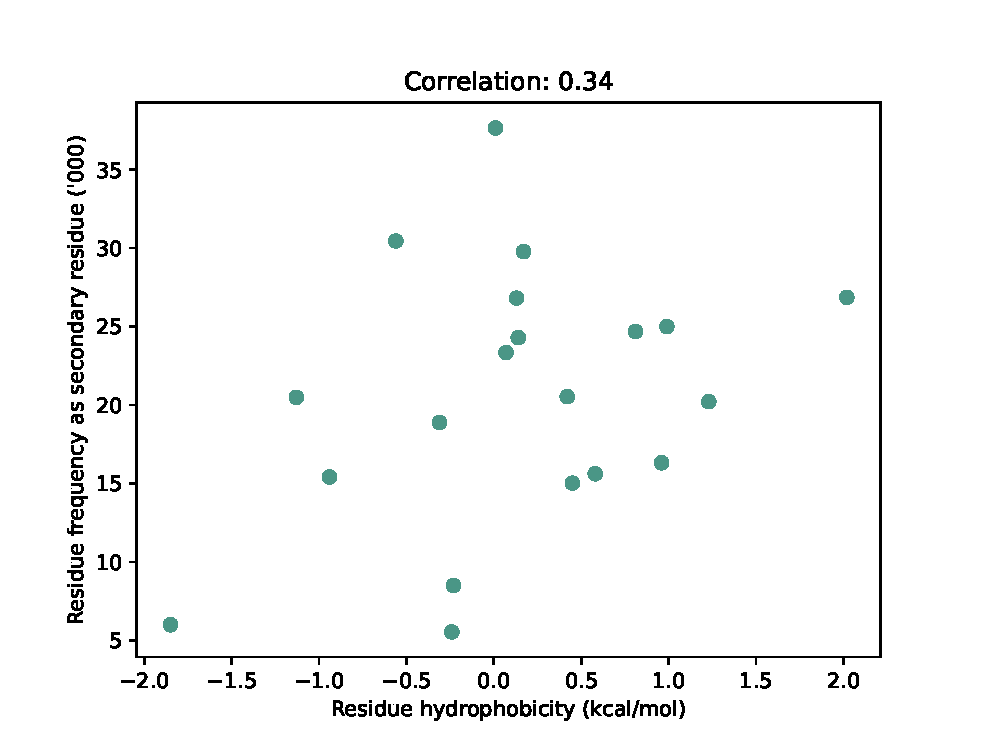
\includegraphics[width=1.0\textwidth]{Figures/secondary-residues.eps}
\caption[Correlation between residue hydrophobicity and their frequency as a secondary residue in zinc binding sites]{\label{fig:secondary-residues} There is a weak correlation between residue hydrophobicity and their frequency as a secondary residue in zinc binding sites.}
\end{figure}

If the primary binding residues' single letter codes are combined to give an overall `signature' of the binding site, C4 (four cysteine residues) is the most prevalent, with 3,069 of the 17,471 unique binding sites having this arrangement of residues (17.6\%) - followed closely by C3H1, with 2149 (12.3\%). That the most common signature makes up just 17.6\% of the total is indicative of the relatively high diversity in such signatures. Between them, the top ten residue signatures account for just 64.4\% of the total.

Of the 24,200 redundant binding sites that contain just one zinc atom, and which come from structures with resolutions better than 3\AA, the most common mode of coordination is via four liganding atoms: 15,077 examples (62.3\%). 5-coordination and 3-coordination have similar prevalences: 4504 (18.6\%) and 1840 (7.6\%) respectively. It is likely that 3-coordination is being over-represented here as, in practice, many sites which have three liganding atoms in the PDB structure are likely missing a fourth ligand in the form of water, meaning that tetrahedral geometry is probably even more widespread than suggested here.

This same subset of binding sites can be used to investigate liganding atom distances. Nitrogen and sulphur atoms both have characteristic distances with tight distributions: $2.12\pm0.16$\AA\ and $2.34\pm0.12$\AA\ respectively. Oxygen however has a much wider distribution, as it can be provided by either of the carboxylate oxygens of the acidic side chains, or from water, with the angle of these two atoms varying continuously. Its average distance to zinc is $2.29\pm0.22$\AA. Overall the average metal-ligand distance is $2.25\pm0.24$\AA  (see Figure~\ref{fig:atom-distances})

\begin{figure}
\centering
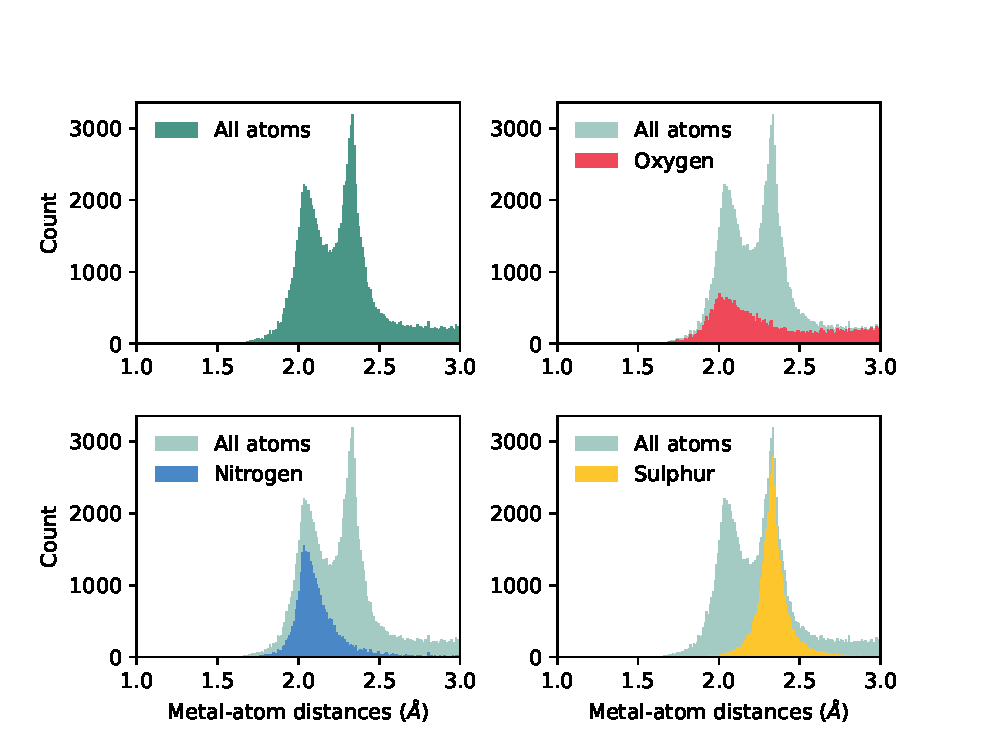
\includegraphics[width=1.0\textwidth]{Figures/atom-distances.eps}
\caption[The distribution of liganding atom distances in all single-zinc sites.]{\label{fig:atom-distances} The distribution of liganding atom
  distances in all single-zinc sites, with a resolution better than
  3\AA. The overall distribution can be seen as bimodal, with the
  first peak being the preferred distance of nitrogen and oxygen, and
  the second peak being the preferred distance of sulphur, which has a
  greater Van der Waals radius.  While nitrogen and sulphur both have
  tight distributions, oxygen does not, and has a much more prominent
  tail in its distribution.}
\end{figure}

\subsection{Co-active Binding Sites}

In some cases multiple metals act in concert to form a single functional unit. Such sites are generally referred to as co-active binding sites in the literature (or `co-catalytic' where the site is known to have a catalytic function). Here, such sites are defined as those instances where a single residue is liganded to more than one metal, according to the criteria defined above. The metals are organised into a single site as described in the methods.

In ZincBind, 3976 from the total of 38,035 zinc binding sites (12.7\%) contain multiple metals: 3550 contain two metals, 394 contain three, 22 contain four, two contain five, and eight zinc binding sites contain six metals (though two of these are from a synthetic construct). In some cases these are binding sites with multiple zinc atoms, but in others the zinc is acting in concert with other metals. Potassium is the most common, represented 319 times, followed by iron (188) and copper (155).

These multi-metal sites account for all of the non-zinc metals in the ZincBind database. While the term `co-catalytic' is sometimes used interchangeably with `co-active', only 83.6\% are derived from an enzymatic protein (defined here as a protein name ending in \emph{--ase}). However this compares with just 61.1\% of all zinc-only binding sites that are enzymatic. A Fisher exact test showed the difference to be significant ($p<0.00001$).

\section{Conclusion}

ZincBind is a database of zinc binding sites --- as such it is both a valuable dataset for this PhD, in the sense that it will serve as training data for predictive models of zinc binding (see next chapter), but it is also a useful resource in its own right. It is is publicly accessible, with a modern GraphQL API and responsive website providing access to the data. The data itself is continuously and automatically updated, and has charactersitics broadly in line with previously observed properties of zinc and other metal binding sites in previous, smaller datasets.

The remainder of this thesis will focus on the dataset's role as a training set for predictive models.